\documentclass[a4paper,oneside]{extbook}
\usepackage{tocloft}

\usepackage{setspace}
\usepackage{indentfirst}
\usepackage{ragged2e}
\usepackage[fontsize=13pt]{scrextend}
\usepackage{enumitem}
\usepackage{lipsum}
\usepackage{longtable}
\usepackage{etoolbox}
\usepackage{lipsum}  % Để tạo văn bản mẫu

\usepackage{tabularx}

% Dãn dòng 1.2
\setstretch{1.2}

% Văn bản canh đều
\justifying

% Thiết lập đoạn
\usepackage{parskip}
\setlength{\parskip}{6pt}

\usepackage[utf8]{vietnam}
%\usepackage{times}
\usepackage{graphicx}
\usepackage{hyperref}
\usepackage{array}
\usepackage{caption}
\usepackage{subcaption}
\usepackage{multirow}
\usepackage{listings}
\usepackage{xcolor}

% custom colors
\definecolor{halfgray}{gray}{0.55}
\definecolor{frame}{RGB}{207, 207, 207}
\definecolor{background}{RGB}{247, 247, 247}
\definecolor{TSX-keyword}{RGB}{42,0.0,255}
\definecolor{TSX-string}{RGB}{127,0,85}
\colorlet{TSX-number}{magenta!60!black}
\definecolor{TSX-comment}{rgb}{0,0.5,0}
\colorlet{TSX-punct}{red!60!black}
\definecolor{TSX-obj-brace}{RGB}{20,105,176}
\definecolor{TSX-lst-brace}{RGB}{20,105,176}
\definecolor{TSX-jsx-tag}{RGB}{0,0,255}

% TypeScript JSX language definition
\lstdefinelanguage{TSX}{
    % common to all of TypeScript
    keywords=[1]{typeof, new, true, false, catch, function, return, null, const, let, var, if, catch, switch, in, while, do, else, case, break, class, export, boolean, throw, implements, import, this, default, async, await, extends, static, get, set, interface, type, public, private, protected, enum, namespace, declare, module},
    % react hooks
    keywords=[2]{useEffect, useState, useRef, useCallback, useMemo, useLayoutEffect, useReducer, useContext, useImperativeHandle, useDebugValue},
    % JSX tags
    keywords=[3]{div, span, h1, h2, h3, h4, h5, h6, p, a, img, ul, li, ol, table, tr, td, th, form, input, button, select, option, textarea, header, footer, nav, section, article, aside, main, figure, figcaption, time, mark, code, pre, blockquote, q, cite, em, strong, small, sub, sup, bdi, bdo, br, wbr, abbr, data, meter, progress, output, details, summary, command, datalist, keygen, menuitem},
    % comments and strings
    comment=[l]{//},
    morecomment=[s]{/*}{*/},
    sensitive=true,     % should be case-sensitive
    morestring=[b]',
    morestring=[b]"
}

% style definition
\lstdefinestyle{TSX}{
    % language grammar
    language=TSX,
    % formatting and styling
    keepspaces=true,
    showspaces=false,
    showstringspaces=false,
    rulecolor=\color{frame},
    frame=single,
    frameround={t}{t}{t}{t},
    framexleftmargin=6mm,
    numbers=left,
    xleftmargin=20pt,
    numberstyle=\tiny\color{halfgray},
    backgroundcolor=\color{background},
    basicstyle=\scriptsize\ttfamily,
    breakatwhitespace=false,         
    breaklines=true,                 
    captionpos=b,                                     
    numbers=left,                    
    numbersep=8pt,                              
    showtabs=false,                  
    tabsize=2,
    stepnumber=1,
    escapeinside={(*!}{!*)},
    % colors and other styles    
    commentstyle=\color{TSX-comment},
    keywordstyle=\color{TSX-keyword},
    keywordstyle=[2]\color{TSX-jsx-tag},
    keywordstyle=[3]\color{TSX-keyword},
    stringstyle=\color{TSX-string},
    literate=
        *{0}{{{\color{TSX-number}0}}}{1}
        {1}{{{\color{TSX-number}1}}}{1}
        {2}{{{\color{TSX-number}2}}}{1}
        {3}{{{\color{TSX-number}3}}}{1}
        {4}{{{\color{TSX-number}4}}}{1}
        {5}{{{\color{TSX-number}5}}}{1}
        {6}{{{\color{TSX-number}6}}}{1}
        {7}{{{\color{TSX-number}7}}}{1}
        {8}{{{\color{TSX-number}8}}}{1}
        {9}{{{\color{TSX-number}9}}}{1}
        {:}{{{\color{TSX-punct}:}}}{1}
        {,}{{{\color{TSX-punct},}}}{1}
        {\{}{{{\color{TSX-obj-brace}{\{}}}}{1}
        {\}}{{{\color{TSX-obj-brace}{\}}}}}{1}
        {[}{{{\color{TSX-lst-brace}{[}}}}{1}
        {]}{{{\color{TSX-lst-brace}{]}}}}{1},
}

\lstset{style=TSX}

\usepackage{mathptmx}
\usepackage{fancyhdr}
\usepackage{algorithm2e}
\usepackage{multicol}
\usepackage{float}

\usepackage{titlesec}

\usepackage{bkthesis}

\title{HỆ THỐNG TỰ ĐỘNG HÓA TRUYỀN THÔNG VÀ THƯƠNG MẠI ĐIỆN TỬ CHO DOANH NGHIỆP ỨNG DỤNG CHATBOT ZALO}
% \csCouncil{KHOA CÔNG NGHỆ THÔNG TIN}
\csSupervise{\textbf{THS. NGUYỄN THỊ HỒNG YẾN}}

\cstuname{%
  \textbf{ĐỖ MỸ XUYÊN}
}
\mssv{%
  \textbf{2101057}
}


\cttime{10/2025}
\thesislayout

% \renewcommand{\thechapter}{\Roman{chapter}}

% Thiết lập định dạng cho \chapter
\titleformat{\chapter}[block]{\normalfont\fontsize{24pt}{24pt}\bfseries\centering}{CHƯƠNG \thechapter:}{1em}{}

\titlespacing*{\chapter}{0pt}{6pt}{0pt}

% Thiết lập định dạng cho \section
\titleformat{\section}[hang]{\normalfont\Large\bfseries}{\thesection}{1em}{}[]

% Khoảng trắng cho \section
\titlespacing*{\section}{0pt}{6pt}{0pt}

% Thiết lập định dạng cho \subsection
\titleformat{\subsection}[hang]{\normalfont\large\bfseries}{\thesubsection}{1em}{}[]

% Khoảng trắng cho \subsection
\titlespacing*{\subsection}{0pt}{6pt}{0pt}

% Thiết lập định dạng cho \subsubsection
\titleformat{\subsubsection}[hang]{\normalfont\normalsize\bfseries}{\thesubsubsection}{1em}{}[]

% Khoảng trắng cho \subsubsection
\titlespacing*{\subsubsection}{0pt}{6pt}{0pt}


\begin{document}
% Thụt đầu dòng 1cm

\captionsetup[figure]{font=bf}
\captionsetup[table]{
  font=bf,
  justification=raggedright,
  singlelinecheck=false
}
\coverpagebandau
\coverpage
\setlength{\parindent}{1cm}
% --- Phần mở đầu, không số trang ---
\begin{declaration}
Tôi xin cam đoan đề tài “Hệ thống Tự động hóa Truyền thông và Thương mại điện tử cho Doanh nghiệp ứng dụng Chatbot Zalo” là kết quả nghiên cứu và thực hiện của tôi dưới sự hướng dẫn của giảng viên hướng dẫn.
Các số liệu, kết quả, nội dung trình bày trong báo cáo đều được thực hiện một cách trung thực, không sao chép từ bất kỳ công trình nào khác. Những tài liệu tham khảo được trích dẫn rõ ràng nguồn gốc theo đúng quy định.
Tôi xin chịu trách nhiệm hoàn toàn về tính chính xác và trung thực của nội dung báo cáo này.


% Signature line
\hfill % pushes the minipage to the right
\begin{minipage}{0.5\textwidth}

\vspace*{1cm} % thụt xuống từ phía trên 3cm

\begin{center}
\textit{Cần Thơ, ngày ... tháng ... năm 2025.} \\
Tác giả đề tài    
\end{center}


\end{minipage}

\end{declaration}                % Lời cam đoan
\begin{acknowledgments}
Trước tiên, tôi xin gửi lời cảm ơn chân thành và sâu sắc nhất đến Ban Giám hiệu Trường Đại học Kỹ Thuật – Công Nghệ Cần Thơ, cùng toàn thể quý Thầy/Cô trong khoa  Công Nghệ Thông Tin đã tận tình giảng dạy, truyền đạt những kiến thức quý báu trong suốt quá trình học tập tại trường.

Đặc biệt, tôi xin chân thành gửi lời cảm ơn đến Th.s Nguyễn Thị Hồng Yến - người Cô đã đồng hành cùng tôi trong đề tài “Hệ thống Tự động hóa Truyền thông và Thương mại điện tử cho Doanh nghiệp ứng dụng Chatbot Zalo”. Cảm ơn Cô đã giúp đỡ và hướng dẫn cho tôi tận tình những lúc tôi gặp khó khăn trong suốt hành trình xây dựng đề tài.

Đây là một trong những cơ hợi giúp tôi phát huy được trình độ và kinh nghiệm trong chuyên ngành của mình. Qua đó, tôi nhận thấy được những ưu điểm và hạn chế của bản thân, từ đó phát huy những điểm mạnh và khắc phục những mặt còn yếu kém. 

Tôi cũng xin gửi lời cảm ơn đến gia đình và bạn bè đã luôn động viên, hỗ trợ tôi cả về tinh thần và vật chất, tạo điều kiện thuận lợi để tôi hoàn thành quá trình nghiên cứu và thực hiện đề tài này.

Trong lúc xây dựng đề tài còn nhiều thiếu sót mong Thầy/Cô nhận xét và góp ý cho tôi để tôi ngày càng hoàn thiện sản phẩm của mình hơn và cũng như hoàn thiện kỹ năng làm việc trong đoạn hành trình sắp tới, một lần nữa tôi xin chân thành cảm ơn Thầy/Cô rất nhiều!

\end{acknowledgments}                % Lời cảm ơn
% \begin{evaluationform}


\end{evaluationform}
       % Phiếu đánh giá (nếu có)
\begin{evaluationteacher}

\vspace{0.2cm}

% Tạo 18 dòng chấm giống hình
\noindent\makebox[\linewidth]{\dotfill}\\[0.5cm]
\noindent\makebox[\linewidth]{\dotfill}\\[0.5cm]
\noindent\makebox[\linewidth]{\dotfill}\\[0.5cm]
\noindent\makebox[\linewidth]{\dotfill}\\[0.5cm]
\noindent\makebox[\linewidth]{\dotfill}\\[0.5cm]
\noindent\makebox[\linewidth]{\dotfill}\\[0.5cm]
\noindent\makebox[\linewidth]{\dotfill}\\[0.5cm]
\noindent\makebox[\linewidth]{\dotfill}\\[0.5cm]
\noindent\makebox[\linewidth]{\dotfill}\\[0.5cm]



\vspace{1cm}

\begin{flushright}
\begin{tabular}{c}
......., ngày....tháng....năm 2025 \\[1em]
\textbf{Giảng viên đánh giá} \\[1em]
\textit{(Ký tên)}
\end{tabular}
\end{flushright}
\end{evaluationteacher} % Xác nhận GV
\begin{tomluoc}
Đề tài thực tập này hướng đến việc nghiên cứu và triển khai 
\textbf{``Hệ thống Tự động hóa Truyền thông và Thương mại Điện tử tích hợp Chatbot Zalo''}. 
Mục tiêu chủ đạo là xây dựng một giải pháp toàn diện, hỗ trợ doanh nghiệp nâng cao hiệu quả trong 
hoạt động \textbf{Marketing}, bán hàng và chăm sóc khách hàng thông qua các công cụ tự động hóa.  

Hệ thống được định hình với ba thành phần trọng tâm:  

\begin{enumerate}
    \item \textbf{Tự động hóa truyền thông}: Thiết kế quy trình tự động tạo ra nội dung truyền thông 
    (video, hình ảnh, bài viết) và lập lịch đăng tải lên các kênh mạng xã hội một cách đồng bộ.
    
    \item \textbf{Website thương mại điện tử}: Phát triển một trang bán điện thoại di động dựa trên 
    nền tảng WordPress, tích hợp đầy đủ các chức năng cơ bản như quản lý sản phẩm, giỏ hàng, đơn hàng 
    và thanh toán.
    
    \item \textbf{Chatbot Zalo}: Xây dựng và cấu hình Chatbot có khả năng tư vấn, trả lời thắc mắc và 
    hỗ trợ khách hàng liên tục 24/7, đồng thời kết nối trực tiếp với hệ thống Website thương mại điện tử.
\end{enumerate}

Trong quá trình triển khai, các công cụ \textbf{N8N} và \textbf{Make.com} được ứng dụng để liên kết và 
tự động hóa toàn bộ quy trình, từ khâu tạo và đăng tải nội dung, quản trị Website đến việc tích hợp dữ liệu 
và giao tiếp qua Chatbot.  

Bên cạnh đó, đề tài còn tập trung đánh giá hiệu quả thực tế của hệ thống trong việc 
\textbf{tiết kiệm chi phí, rút ngắn thời gian vận hành, tăng tính chuyên nghiệp} và 
\textbf{cải thiện trải nghiệm khách hàng}, đặc biệt phù hợp với các \textbf{doanh nghiệp vừa và nhỏ} 
hoạt động trong lĩnh vực kinh doanh sản phẩm công nghệ tại thị trường Việt Nam.  

\end{tomluoc}                % Tóm lược

% --- Bắt đầu frontmatter: số trang La Mã ---
\frontmatter
\pagestyle{plain}  % Số trang i, ii, iii... ở footer giữa

% --- Mục lục, danh mục ---
\renewcommand{\cfttoctitlefont}{\hfil\Large\bfseries}
\renewcommand{\cftaftertoctitle}{\centering}
\renewcommand{\contentsname}{MỤC LỤC}
\tableofcontents
\clearpage

\renewcommand{\cftloftitlefont}{\hfil\Large\bfseries}
\renewcommand{\cftafterloftitle}{\centering}
\renewcommand{\listfigurename}{DANH MỤC HÌNH ẢNH}
\listoffigures
\clearpage

\renewcommand{\cftlottitlefont}{\hfil\Large\bfseries}
\renewcommand{\cftafterlottitle}{\centering}
\renewcommand{\listtablename}{DANH MỤC BẢNG}
% \listoftables
\clearpage

% --- Các phần phụ trước nội dung chính ---
\begin{category}
\begin{center}
\begin{tabular}{|m{3cm}|m{4cm}|m{8cm}|}
\hline
\textbf{Viết tắt} & \textbf{Tiếng Anh} & \textbf{Giải thích / Thuật ngữ} \\
\hline
AI & Artificial Intelligence & Trí tuệ nhân tạo – khả năng máy tính mô phỏng hành vi trí tuệ con người. \\
\hline
API & Application Programming Interface & Giao diện lập trình ứng dụng, cho phép các hệ thống phần mềm giao tiếp với nhau. \\
\hline
CMS & Content Management System & Hệ thống quản lý nội dung, hỗ trợ xây dựng và quản lý website. \\
\hline
TTTN & Thực tập tốt nghiệp & Quá trình sinh viên tham gia thực tập tại doanh nghiệp để tích lũy kinh nghiệm. \\
\hline
ZNS & Zalo Notification Service & Dịch vụ gửi thông báo tự động từ doanh nghiệp đến khách hàng trên Zalo. \\
\hline
NLP & Natural Language Processing & Xử lý ngôn ngữ tự nhiên, giúp Chatbot hiểu và phản hồi văn bản. \\
\hline
UI/UX & User Interface / User Experience & Giao diện và trải nghiệm người dùng trong ứng dụng/website. \\
\hline
SQL & Structured Query Language & Ngôn ngữ truy vấn có cấu trúc, dùng trong quản lý cơ sở dữ liệu. \\
\hline
TTĐH & Tự động hóa & Quá trình sử dụng công nghệ để tự động vận hành quy trình, giảm thiểu thủ công. \\
\hline
N8N & Node-Eight-Node & Nền tảng mã nguồn mở giúp bạn kết nối các ứng dụng, dịch vụ và API lại với nhau. \\
\hline
\end{tabular}
\end{center}

\end{category}               % Danh mục viết tắt
\begin{abstract}
\section{LÍ DO CHỌN ĐỀ TÀI}
Trong bối cảnh chuyển đổi số đang diễn ra mạnh mẽ, các doanh nghiệp ngày càng
chú trọng đến việc tối ưu hoá hoạt động truyền thông và thương mại điện tử nhằm nâng
cao hiệu quả kinh doanh. Zalo hiện là một trong những nền tảng mạng xã hội phổ biến
tại Việt Nam, với lượng người dùng lớn và mức độ tương tác cao. Việc ứng dụng Chatbot
Zalo giúp doanh nghiệp tự động hóa quá trình chăm sóc khách hàng, quảng bá sản phẩm,
xử lý đơn hàng và hỗ trợ bán hàng 24/7, từ đó tiết kiệm chi phí, giảm tải nhân sự và nâng
cao trải nghiệm khách hàng.
Xuất phát từ nhu cầu thực tiễn đó, đề tài “Hệ thống tự động hóa truyền thông và
thương mại điện tử cho doanh nghiệp ứng dụng Chatbot Zalo” được lựa chọn với mong
muốn nghiên cứu, xây dựng giải pháp ứng dụng công nghệ vào hoạt động kinh doanh,
hỗ trợ doanh nghiệp mở rộng thị trường, tăng khả năng cạnh tranh và bắt kịp xu hướng
số hóa.
\section{MỤC TIÊU VÀ PHẠM VI THỰC TẬP}
\subsection{Mục tiêu} 
Thông qua đề tài “Hệ thống Tự động hóa Truyền thông và Thương mại Điện tử cho Doanh nghiệp ứng dụng Chatbot Zalo”, tôi mong muốn đạt được:  

\begin{itemize}
    \item \textbf{Tự động hóa quy trình truyền thông}: Giúp doanh nghiệp dễ dàng đăng tải, quản lý và phân phối nội dung trên nhiều kênh khác nhau, từ đó tiết kiệm thời gian và nhân lực.
    \item \textbf{Nâng cao hiệu quả chăm sóc khách hàng}: Ứng dụng Chatbot Zalo nhằm phản hồi khách hàng nhanh chóng, chính xác, hỗ trợ 24/7, cải thiện trải nghiệm và tăng mức độ hài lòng.
    \item \textbf{Hỗ trợ bán hàng trực tuyến}: Cung cấp kênh tư vấn, giới thiệu sản phẩm và xử lý đơn hàng trực tiếp trên nền tảng Zalo, góp phần thúc đẩy doanh số bán hàng.
    \item \textbf{Tối ưu chi phí và nguồn lực}: Giúp doanh nghiệp, đặc biệt là doanh nghiệp vừa và nhỏ, tiết kiệm chi phí vận hành và giảm tải công việc lặp lại cho nhân sự.
    \item \textbf{Nâng cao năng lực cạnh tranh}: Tạo lợi thế cho doanh nghiệp trong xu thế chuyển đổi số, bắt kịp các xu hướng công nghệ mới và mở rộng thị trường kinh doanh.
\end{itemize}

\subsection{Phạm vi thực hiện} 
\begin{itemize}
    \item \textbf{Địa điểm}: Thành phố Cần Thơ.  
    \item \textbf{Đối tượng nghiên cứu}: Hệ thống Chatbot Zalo và các công cụ hỗ trợ truyền thông, chăm sóc khách hàng, thương mại điện tử.  
    \item \textbf{Thời gian}: Dự kiến kéo dài trong 3–4 tháng.  
\end{itemize}
\section{PHƯƠNG PHÁP NGHIÊN CỨU}
Nghiên cứu này sẽ tập trung vào việc xây dựng và triển khai một hệ thống tích hợp, bao gồm các khía cạnh sau:

\begin{itemize}
    \subsection{Về công nghệ và nền tảng:}
    \begin{itemize}
        \item {Tự động hóa:} Sử dụng các công cụ N8N và Make.com để thiết lập các luồng tự động hóa quy trình.
        \item {Website Thương mại điện tử:} Xây dựng trên nền tảng WordPress kết hợp với các Plugin phù hợp (ví dụ: WooCommerce).
        \item {Chatbot:} Tích hợp và cấu hình Chatbot trên nền tảng Zalo, sử dụng Zalo API để tương tác.
        \item {Nền tảng truyền thông:} Kết nối với các API của các mạng xã hội phổ biến (ví dụ: Facebook Fanpage, Instagram, TikTok) để tự động đăng tải nội dung.
    \end{itemize}

    \subsection{Về chức năng hệ thống:}
    \begin{itemize}
        \item{Tạo và đăng tải nội dung tự động:} Phát triển mô hình tự động tạo video, hình ảnh marketing và bài viết, sau đó tự động đăng lên các kênh mạng xã hội theo lịch trình.
        \item {Quản lý sản phẩm và bán hàng:} Triển khai Website bán điện thoại với các chức năng cơ bản của thương mại điện tử (hiển thị sản phẩm, giỏ hàng, đặt hàng, quản lý đơn hàng đơn giản).
        \item {Chăm sóc khách hàng tự động:} Chatbot Zalo có khả năng giải đáp các câu hỏi thường gặp, tư vấn thông tin sản phẩm (mô tả, giá, tình trạng hàng), và hỗ trợ các yêu cầu cơ bản từ khách hàng.
    \end{itemize}

    \subsection{Về đối tượng và giới hạn:}
    \begin{itemize}
        \item{Đối tượng ứng dụng:} Tập trung vào các doanh nghiệp vừa và nhỏ (SMEs) hoạt động trong lĩnh vực bán lẻ sản phẩm công nghệ, đặc biệt là điện thoại di động.
        \item {Giới hạn:} Nghiên cứu sẽ tập trung vào việc tích hợp các công cụ và nền tảng có sẵn để xây dựng hệ thống tự động hóa. Đề tài không đi sâu vào việc phát triển các thuật toán AI hoặc Engine Chatbot từ đầu mà sẽ tận dụng các giải pháp API và công cụ no-code/low-code hiện có. Hệ thống thanh toán và vận chuyển sẽ được tích hợp ở mức cơ bản hoặc giả lập tùy theo khả năng triển khai trong phạm vi thực tập.
    \end{itemize}
\end{itemize}
\section{BỐ CỤC BÀI VIẾT}
Đồ án thực tập bao gồm 4 chương:
\begin{itemize}
    \item Chương 1: GIỚI THIỆU TỔNG QUAN.
    \item Chương 2: TỔNG QUAN VỀ CƠ SỞ LÝ THUYẾT
    \item Chương 3: KẾT QUẢ - THẢO LUẬN.
    \item Chương 4: KẾT LUẬN VÀ ĐỀ XUẤT (KIẾN NGHỊ).
\end{itemize}
\end{abstract}                % Lời mở đầu
\include{TheReason}                 % Lí do chọn đề tài
\include{Theobjectivesandscope}     % Mục tiêu và phạm vi
\include{Thephuongphap}             % Phương pháp nghiên cứu

% --- Bắt đầu mainmatter: số trang Ả Rập ---
\mainmatter
% \pagestyle{fancy}   % Bật header/footer fancy
% \fancyhf{}          % Xóa header/footer cũ
% \fancyfoot[C]{\thepage} % Số trang ở giữa footer
% \fancyhead[L]{\nouppercase{\leftmark}} % Header trái: tên chương
% \fancyhead[R]{\nouppercase{\rightmark}} % Header phải: tên section

% --- Nội dung chính ---
\chapter{GIỚI THIỆU TỔNG QUAN}
\section{THÔNG TIN VỀ ĐƠN VỊ THỰC TẬP}
\subsection{ Sơ lược về sự hình thành và phát triển của đơn vị}
Công ty Cổ phần Bảo vệ Thực vật Delta (Delta Corp.) bắt đầu tham gia vào lĩnh vực nông nghiệp từ năm 2009 và không ngừng nỗ lực để khẳng định vị thế của mình trong ngành nông nghiệp Việt Nam. Với tầm nhìn dài hạn và chiến lược phát triển bền vững, công ty chuyên phân phối các mặt hàng thuốc bảo vệ thực vật và sản xuất phân bón trung vi lượng phục vụ trực tiếp cho bà con nông dân. \\
\indent Qua nhiều năm hoạt động, công ty giữ vững phương châm \textit{``Chất lượng sản phẩm là uy tín – Sự hài lòng của khách hàng là thành công''}, đồng thời liên tục mở rộng quy mô sản phẩm từ thuốc đặc trị đến các dòng phân bón dưỡng cây. Các sản phẩm đã phủ sóng tại Đồng bằng sông Cửu Long, miền Đông Nam Bộ và Tây Nguyên, góp phần cải thiện năng suất mùa vụ. \\
\indent Hiện tại, Delta sở hữu gần 50 cán bộ – nhân viên, với môi trường làm việc chuyên nghiệp, đoàn kết, cùng nhau xây dựng mục tiêu phát triển bền vững theo tinh thần:
\begin{itemize}
    \item ``Đóng góp nhỏ – Gặt hái to''.
    \item ``Phát triển nội lực – Vững bước tương lai''.
\end{itemize}

\subsection{ Tổ chức và các lĩnh vực hoạt động của đơn vị}
Hiện nay, các sản phẩm của Delta được phân phối rộng rãi tại nhiều tỉnh thành, đặc biệt là Đồng bằng Sông Cửu Long, miền Đông Nam Bộ và Tây Nguyên. Trong 5 năm tới, Delta định hướng mở rộng thị trường ra miền Trung và miền Bắc, đồng thời chú trọng nghiên cứu các dòng chế phẩm sinh học hướng tới tiêu chí ``Môi trường xanh – sản phẩm sạch''. \\
\indent Bên cạnh thị trường và sản phẩm, công ty cũng chú trọng đào tạo nhân sự, xây dựng đội ngũ vững mạnh cả về chuyên môn lẫn đạo đức nghề nghiệp.

\subsection{ Tổ chức quản lý và sử dụng các nguồn lực của đơn vị}
\subsubsection{a. Nguồn nhân lực}
Delta hiện có gần 50 cán bộ – nhân viên, phân bổ tại các phòng ban: Ban Giám đốc, Phòng Kinh doanh, Phòng Kỹ thuật, Phòng Công Nghệ Thông Tin, Phòng Nghiên cứu \& Phát triển, Phòng Hành chính – Nhân sự, Phòng Kế toán – Tài chính và Đội ngũ thị trường. Công ty chú trọng đào tạo, bồi dưỡng kỹ năng và giữ chân nhân tài.
\subsubsection*{b. Nguồn lực tài chính}
Nguồn vốn ổn định, đảm bảo sản xuất – kinh doanh, phân bổ hợp lý cho đầu tư công nghệ, nghiên cứu sản phẩm, Marketing và đãi ngộ nhân sự.
\subsubsection*{b. Nguồn lực vật chất – kỹ thuật}
Sở hữu nhà máy sản xuất phân bón hiện đại, hệ thống kho bãi đạt chuẩn và phương tiện vận chuyển chuyên dụng.
\subsubsection*{c. Nguồn lực công nghệ – thông tin}
Ứng dụng phần mềm quản lý kho, bán hàng, kế toán, CRM và nền tảng số ( Zalo OA, Website, Fanpage) để tăng hiệu quả vận hành.
\subsubsection*{d. Nguồn lực quan hệ – thị trường}
Mạng lưới hơn 300 đại lý và nhà phân phối, hợp tác với chuyên gia nông nghiệp và tổ chức bảo vệ thực vật để cải tiến sản phẩm.

\subsection{ Cơ cấu tổ chức}
Bộ máy quản lý gồm Ban Giám đốc, Phòng Kinh doanh, Phòng CNTT, Phòng Kỹ thuật – Tư vấn, Phòng R\&D, Hành chính – Nhân sự, Kế toán – Tài chính, và Xưởng sản xuất – kho vận. Các phòng ban phối hợp chặt chẽ, đảm bảo hoạt động trơn tru từ nghiên cứu, sản xuất, phân phối đến chăm sóc khách hàng.

\subsection{ Mô tả sơ đồ hoạt động}
Quy trình hoạt động của Delta bao gồm:
\begin{itemize}
    \item Nghiên cứu sản phẩm mới.
    \item Sản xuất – kiểm định chất lượng.
    \item Phân phối – tiếp cận thị trường.
    \item Chăm sóc khách hàng – hậu mãi.
    \item Phản hồi – cải tiến sản phẩm và dịch vụ.
\end{itemize}

\subsection{ Năng lực sản xuất – phát triển sản phẩm}
Delta có công suất sản xuất 1.000–1.500 tấn/tháng, với hơn 300 dòng phân bón và 100 dòng thuốc bảo vệ thực vật. Công ty liên tục cải tiến công thức, hợp tác với chuyên gia, đồng thời tổ chức hội thảo đầu bờ giúp bà con nông dân tiếp cận và sử dụng hiệu quả sản phẩm. Delta hướng tới mở rộng thị trường trong nước và quốc tế, phát triển bền vững và thân thiện môi trường.
\section{THÔNG TIN VỀ CÔNG VIỆC THỰC TẬP}
Trong quá trình thực tập, sinh viên được giao các công việc liên quan đến lĩnh vực công nghệ thông tin và truyền thông số, cụ thể như sau:

\begin{itemize}
    \item \textbf{Tìm hiểu và nghiên cứu nhu cầu truyền thông số của công ty:} 
    Phân tích hiện trạng hoạt động kinh doanh, nhận thấy công ty chủ yếu bán hàng qua hệ thống đại lý, các kênh trực tuyến chưa được khai thác hiệu quả.
    
    \item \textbf{Đề xuất xây dựng hệ thống kênh truyền thông đa nền tảng:} 
    Bao gồm Zalo Official Account, Facebook Fanpage và Website WordPress để tăng khả năng tiếp cận khách hàng.
    
    \item \textbf{Thiết kế và triển khai Chatbot Zalo:}
    \begin{itemize}
        \item Tự động trả lời câu hỏi về sản phẩm (phân bón, thuốc bảo vệ thực vật).
        \item Gửi tin nhắn quảng bá theo từng chiến dịch Marketing.
        \item Hỗ trợ khách hàng đặt hàng nhanh và chốt đơn tự động.
        \item Kết nối Chatbot với cơ sở dữ liệu sản phẩm của công ty.
    \end{itemize}
    
    \item \textbf{Phát triển nội dung truyền thông:}
    \begin{itemize}
        \item Biên tập và xử lý Video quảng cáo (giới thiệu sản phẩm, hướng dẫn sử dụng) để đăng tải trên Facebook Fanpage.
        \item Thiết kế hình ảnh truyền thông (Poster, Banner, Infographic) bằng Canva/Photoshop và đăng tải trên Website WordPress.
        \item Tối ưu nội dung chuẩn SEO để tăng hiển thị trên Google.
    \end{itemize}
    
    \item \textbf{Xây dựng hệ thống thương mại điện tử tích hợp:}
    \begin{itemize}
        \item Kết nối Chatbot Zalo với hệ thống quản lý đơn hàng.
        \item Tự động hóa việc gửi thông tin đơn hàng từ Zalo về Email hoặc phần mềm quản lý bán hàng.
        \item Hỗ trợ xây dựng giao diện bán hàng trên WordPress (giới thiệu sản phẩm, Form đặt hàng trực tuyến).
    \end{itemize}
    
    \item \textbf{Báo cáo – đánh giá hiệu quả:}
    \begin{itemize}
        \item Thống kê số lượng khách hàng tương tác với Chatbot.
        \item Đánh giá hiệu quả Video quảng cáo trên Facebook (Reach, lượt xem, tương tác).
        \item Đo lường mức độ quan tâm của khách hàng từ Website WordPress.
    \end{itemize}
\section{NỘI QUY AN TOÀN - VỆ SINH LAO ĐỘNG}
\begin{itemize}
    \subsection{Quy định chung:}
    \begin{itemize}
        \item Giữ gìn trật tự, vệ sinh trong phòng làm việc; không ăn uống gần khu vực máy tính, thiết bị mạng.
        \item Sử dụng thiết bị đúng mục đích, không tự ý di chuyển, tháo lắp máy tính hoặc linh kiện khi chưa có sự cho phép.
        \item Luôn tuân thủ giờ giấc làm việc, tôn trọng không gian làm việc chung.
    \end{itemize}

    \subsection{An toàn trong sử dụng thiết bị CNTT:}
    \begin{itemize}
        \item Kiểm tra dây nguồn, thiết bị ngoại vi trước khi sử dụng; tắt máy tính đúng quy trình khi kết thúc công việc.
        \item Không cài đặt phần mềm lạ, không rõ nguồn gốc lên hệ thống của công ty.
        \item Đảm bảo an toàn thông tin: không chia sẻ tài khoản, mật khẩu hoặc dữ liệu nội bộ ra bên ngoài.
    \end{itemize}

    \subsection{Quy định khi bảo trì và lắp ráp thiết bị:}
    \begin{itemize}
        \item Ngắt nguồn điện trước khi tháo lắp, thay thế linh kiện máy tính hoặc thiết bị mạng.
        \item Sử dụng đúng dụng cụ được cấp khi bảo trì, không sử dụng thiết bị cá nhân không đạt chuẩn.
        \item Chỉ thực hiện các công việc kỹ thuật dưới sự hướng dẫn của cán bộ phụ trách.
    \end{itemize}

    \subsection{An toàn tại nơi làm việc:}
    \begin{itemize}
        \item Không để vật cản chắn lối đi, đảm bảo lối thoát hiểm luôn thông thoáng.
        \item Thực hiện phân loại rác thải (rác thải sinh hoạt, rác thải điện tử) đúng quy định.
        \item Giữ thái độ làm việc chuyên nghiệp, hỗ trợ đồng nghiệp khi cần thiết.
    \end{itemize}
\end{itemize}
\end{itemize}
\section{THÔNG TIN LIÊN HỆ}
\begin{itemize}
    \item \textbf{Địa chỉ:} 132K, đường Nguyễn Văn Cừ, Phường An Khánh, Quận Ninh Kiều, Thành Phố Cần Thơ.
    \item \textbf{Địa chỉ:} 0827 26 27 28
\end{itemize}


\chapter{TỔNG QUAN VỀ CƠ SỞ LÝ THUYẾT}
\section{LƯỢC KHẢO TÀI LIỆU}  
\subsection{Nghiên cứu về Chatbot trong thương mại điện tử}
Chatbot là một trong những giải pháp công nghệ nổi bật, được ứng dụng rộng rãi nhằm tự động hóa giao tiếp giữa doanh nghiệp và khách hàng. Theo nhiều nghiên cứu gần đây, chatbot có thể thay thế một phần công việc của đội ngũ chăm sóc khách hàng, cung cấp dịch vụ 24/7, giảm tải chi phí vận hành và nâng cao trải nghiệm người dùng. Các nền tảng thương mại điện tử lớn như Amazon, Alibaba hay Shopee đều đã triển khai Chatbot để hỗ trợ tra cứu thông tin sản phẩm, xử lý đơn hàng và chăm sóc sau bán.  

Tại Việt Nam, nhiều doanh nghiệp nhỏ và vừa cũng đã bước đầu ứng dụng chatbot, đặc biệt trên các nền tảng mạng xã hội như Facebook Messenger. Tuy nhiên, việc khai thác chatbot trên các nền tảng bản địa, điển hình là Zalo, vẫn chưa được nghiên cứu và triển khai rộng rãi.  

\subsection{Nghiên cứu và ứng dụng Zalo Chatbot}
Zalo hiện là mạng xã hội có lượng người dùng lớn tại Việt Nam, với ưu thế mạnh mẽ trong giao tiếp và thương mại nội địa. Từ năm 2018, Zalo đã mở API cho phép phát triển chatbot, hỗ trợ doanh nghiệp xây dựng hệ thống tư vấn và chăm sóc khách hàng tự động. Một số nghiên cứu bước đầu cho thấy chatbot Zalo giúp doanh nghiệp Việt Nam tiếp cận khách hàng nhanh chóng hơn, đặc biệt trong các lĩnh vực bán lẻ, thương mại điện tử và dịch vụ công.  

Tuy vậy, phần lớn ứng dụng mới dừng lại ở các chức năng cơ bản như trả lời tin nhắn tự động hoặc gửi thông báo đơn hàng. Việc tích hợp sâu hơn chatbot Zalo với các hệ thống thương mại điện tử và công cụ marketing vẫn còn hạn chế, tạo ra khoảng trống cho các nghiên cứu và giải pháp ứng dụng thực tiễn.  

\subsection{Các nền tảng công nghệ hỗ trợ tự động hóa}
Song song với sự phát triển của chatbot, nhiều nền tảng hỗ trợ tự động hóa quy trình truyền thông và kinh doanh cũng được quan tâm. Các công cụ như \textbf{N8N} và \textbf{Make.com} cho phép xây dựng workflow tự động, liên kết nhiều ứng dụng với nhau (ví dụ: tạo nội dung $\rightarrow$ xử lý $\rightarrow$ đăng tải lên mạng xã hội). Trong khi đó, \textbf{WordPress} kết hợp với \textbf{WooCommerce} được sử dụng phổ biến để xây dựng website thương mại điện tử cho doanh nghiệp vừa và nhỏ nhờ tính dễ triển khai và chi phí thấp.  

Việc kết hợp các nền tảng này giúp doanh nghiệp tối ưu hóa toàn bộ chuỗi hoạt động: từ quản lý dữ liệu, tự động tạo nội dung, vận hành website, đến chăm sóc khách hàng thông qua chatbot.  

\subsection{Đánh giá và khoảng trống nghiên cứu}
Qua lược khảo, có thể thấy các nghiên cứu và ứng dụng hiện nay tập trung mạnh vào \textbf{chatbot trên Facebook Messenger} và các giải pháp thương mại điện tử truyền thống. Trong khi đó, \textbf{Zalo Chatbot}, một nền tảng có lợi thế tại thị trường Việt Nam, vẫn chưa được khai thác toàn diện. Bên cạnh đó, việc tích hợp đồng bộ \textbf{Chatbot Zalo – Website thương mại điện tử – Hệ thống tự động hóa truyền thông} chưa có nhiều nghiên cứu cụ thể.  

Chính vì vậy, đề tài ``\textit{Hệ thống Tự động hóa Truyền thông và Thương mại Điện tử cho Doanh nghiệp ứng dụng Chatbot Zalo}'' được thực hiện với mong muốn bổ sung vào khoảng trống này. Đề tài không chỉ mang ý nghĩa học thuật trong việc áp dụng công nghệ mới, mà còn có giá trị thực tiễn cao đối với doanh nghiệp vừa và nhỏ tại Việt Nam trong bối cảnh số hóa hiện nay.  

\section{CƠ SỞ LÝ THUYẾT}

\subsection{Google Sheets và Google Drive – nền tảng lưu trữ và quản lý dữ liệu trên đám mây}

\textbf{Định nghĩa:}
\begin{itemize}
    \item \textbf{Google Sheets} là ứng dụng bảng tính trực tuyến do Google phát triển, hoạt động trên nền tảng Web và đồng bộ với Google Drive. Sheets cho phép nhiều người dùng cùng tạo, chỉnh sửa và cộng tác trên một bảng tính theo thời gian thực.
    \item \textbf{Google Drive} là dịch vụ lưu trữ và đồng bộ tệp trên đám mây, cho phép tải lên, chia sẻ và truy cập tài liệu, hình ảnh, video từ bất kỳ thiết bị nào.
\end{itemize}

Trong hệ thống, Google Sheets được dùng để quản lý dữ liệu thương hiệu và sản phẩm, còn Google Drive lưu trữ hình ảnh/Video để Chatbot và hệ thống tự động hóa có thể sử dụng khi cần.

\textbf{Thành phần/Cấu trúc chính:}
\begin{itemize}
    \item \textbf{Google Sheets:}
    \begin{itemize}
        \item Cell/Row/Column: đơn vị cơ bản.
        \item Function \& Formula: tính toán, xử lý dữ liệu.
        \item Collaboration: nhiều người chỉnh sửa cùng lúc.
        \item Integration API: kết nối Make.com, N8N, AI.
    \end{itemize}
    \item \textbf{Google Drive:}
    \begin{itemize}
        \item File Storage: lưu nhiều định dạng.
        \item Folder Structure: tổ chức khoa học.
        \item Permission \& Sharing: quản lý quyền truy cập.
        \item API Access: ứng dụng có thể lấy/cập nhật dữ liệu.
    \end{itemize}
\end{itemize}

\textbf{Ứng dụng trong thực tiễn (KingPhone):}
\begin{itemize}
    \item Google Sheets: lưu thông tin thương hiệu, sản phẩm; nguồn dữ liệu đầu vào cho AI; kết nối với N8N để chatbot Zalo gửi Menu.
    \item Google Drive: lưu hình ảnh sản phẩm, Video Marketing để đăng tải lên YouTube, Fanpage.
\end{itemize}

\textbf{Ưu điểm:}
\begin{itemize}
    \item Miễn phí/chi phí thấp.
    \item Cộng tác theo thời gian thực.
    \item Tích hợp mạnh mẽ với API.
    \item Đồng bộ đám mây.
    \item Bảo mật với phân quyền chi tiết.
\end{itemize}

\textbf{Nhược điểm:}
\begin{itemize}
    \item Giới hạn dung lượng miễn phí (15GB).
    \item Phụ thuộc Internet.
    \item Bảo mật phụ thuộc người quản trị.
    \item Hiệu suất giảm khi dữ liệu lớn.
\end{itemize}

\textbf{Vai trò trong đề tài:}
\begin{itemize}
    \item Là nguồn dữ liệu trung tâm: Sheets cung cấp dữ liệu, Drive lưu media.
    \item Đảm bảo dữ liệu cập nhật và đồng bộ.
    \item Dễ quản lý, không cần can thiệp mã nguồn.
\end{itemize}

\textbf{Lợi ích:}
\begin{itemize}
    \item Kho dữ liệu linh hoạt, dễ chỉnh sửa.
    \item AI và Chatbot có thể tự động lấy dữ liệu mới nhất.
    \item Tạo sự kết nối chặt chẽ giữa Make.com – N8N – WordPress – Zalo – Fanpage – YouTube.
\end{itemize}

\begin{figure}
\centering
    
\includegraphics[width=0.7\textwidth]{img/gg.png}
    
    \caption{ Hệ sinh thái Google}
    \label{fig:gg}
\end{figure}


%----------------------------------------------------

\subsection{AI (Trí tuệ nhân tạo)}

\textbf{Định nghĩa:} AI là lĩnh vực khoa học máy tính phát triển hệ thống có khả năng mô phỏng trí tuệ con người (học hỏi, suy luận, giải quyết vấn đề, NLP, ra quyết định). Trong đề tài, AI được dùng để tạo nội dung Marketing và xử lý ngôn ngữ tự nhiên cho Chatbot Zalo.

\textbf{Thành phần/Cấu trúc chính:}
\begin{itemize}
    \item Natural Language Processing (NLP).
    \item Generative AI: sinh bài viết, hình ảnh, Video.
    \item Machine Learning Model: học dữ liệu từ Google Sheets.
    \item Integration With Workflow: kết nối Make.com, N8N.
\end{itemize}

\textbf{Ứng dụng:}
\begin{itemize}
    \item Make.com: sinh bài viết, ảnh, Video.
    \item N8N + Zalo API: phân tích tin nhắn, phản hồi tự động, gửi sản phẩm kèm hình ảnh.
\end{itemize}

\textbf{Ưu điểm:}
\begin{itemize}
    \item Tự động hóa sáng tạo nội dung.
    \item Hiểu ngôn ngữ tự nhiên.
    \item Tiết kiệm chi phí, thời gian.
    \item Khả năng mở rộng, linh hoạt.
\end{itemize}

\textbf{Nhược điểm:}
\begin{itemize}
    \item Chi phí API.
    \item Phụ thuộc dữ liệu huấn luyện.
    \item Hạn chế ngữ cảnh phức tạp.
    \item Cần giám sát nội dung sinh ra.
\end{itemize}

\textbf{Vai trò:}
\begin{itemize}
    \item Bộ não thông minh: Make.com sinh nội dung, N8N xử lý NLP cho chatbot.
    \item Đảm bảo hệ thống tự động và thông minh.
\end{itemize}

\textbf{Lợi ích:}
\begin{itemize}
    \item Hệ thống Marketing – chăm sóc khách hàng chuyên nghiệp.
    \item Trải nghiệm tư vấn 24/7.
    \item Nội dung đồng bộ thương hiệu.
\end{itemize}

\begin{figure}
\centering
    
\includegraphics[width=0.8\textwidth]{img/Picture2.png}
    
    \caption{Mô hình AI trong chăm sóc khách hàng}
    \label{fig:chamsoc}
\end{figure}

%----------------------------------------------------

\subsection{Zalo API qua N8N – tích hợp Chatbot}

\textbf{Định nghĩa:} Zalo API được tích hợp qua N8N để giảm độ phức tạp và tăng linh hoạt, phục vụ xây dựng chatbot thương mại điện tử.

\textbf{Thành phần:}
\begin{itemize}
    \item Webhook Trigger Node.
    \item Message Node.
    \item User Node.
    \item Google Sheets/Drive Node.
    \item AI Node (OpenAI).
    \item Database Node.
    \item Admin Flow.
\end{itemize}

\textbf{Ứng dụng (KingPhone):}
\begin{itemize}
    \item Tiếp nhận, phân loại tin nhắn.
    \item Cung cấp menu sản phẩm động.
    \item Tư vấn tự động 24/7.
    \item Đồng bộ với Website TMĐT.
    \item Hỗ trợ quản trị viên.
\end{itemize}

\textbf{Ưu điểm:}
\begin{itemize}
    \item Tích hợp dễ dàng.
    \item Linh hoạt.
    \item Tự động hóa mạnh.
    \item Dữ liệu tập trung.
    \item Phù hợp thị trường Việt Nam.
\end{itemize}

\textbf{Nhược điểm:}
\begin{itemize}
    \item Yêu cầu kỹ năng N8N.
    \item Phụ thuộc Server.
    \item Cần bảo mật tốt Token, dữ liệu.
\end{itemize}

\begin{figure}
    \centering
    
\includegraphics[width=0.7\textwidth]{img/Picture3.png}

    \caption{Zalo API qua N8N trong hệ thống tư vấn khách hàng}
    \label{fig:zaloapi}
\end{figure}

%----------------------------------------------------

\subsection{Make.com – nền tảng tự động hóa quy trình}

\textbf{Định nghĩa:} Make.com (trước đây Integromat) là nền tảng Automation, kết nối ứng dụng, dịch vụ, API bằng giao diện kéo-thả, không cần nhiều Code.

\textbf{Thành phần:}
\begin{itemize}
    \item Scenario.
    \item Module.
    \item Trigger.
    \item Action.
    \item Iterator \& Aggregator.
    \item Error Handler.
\end{itemize}

\textbf{Ứng dụng (KingPhone):}
\begin{itemize}
    \item Sheets nhập dữ liệu thương hiệu.
    \item AI sinh nội dung.
    \item Drive lưu Media.
    \item WordPress, Facebook, YouTube đăng bài.
\end{itemize}

\textbf{Ưu điểm:}
\begin{itemize}
    \item Không cần lập trình nhiều.
    \item Tích hợp linh hoạt.
    \item Tự động hóa mạnh.
    \item Khả năng mở rộng.
    \item Tiết kiệm chi phí.
\end{itemize}

\textbf{Nhược điểm:}
\begin{itemize}
    \item Phụ thuộc Internet.
    \item Thiết lập Workflow phức tạp.
    \item Giới hạn theo gói dịch vụ.
    \item Bảo mật phụ thuộc Cloud.
\end{itemize}

\begin{figure}
\centering
    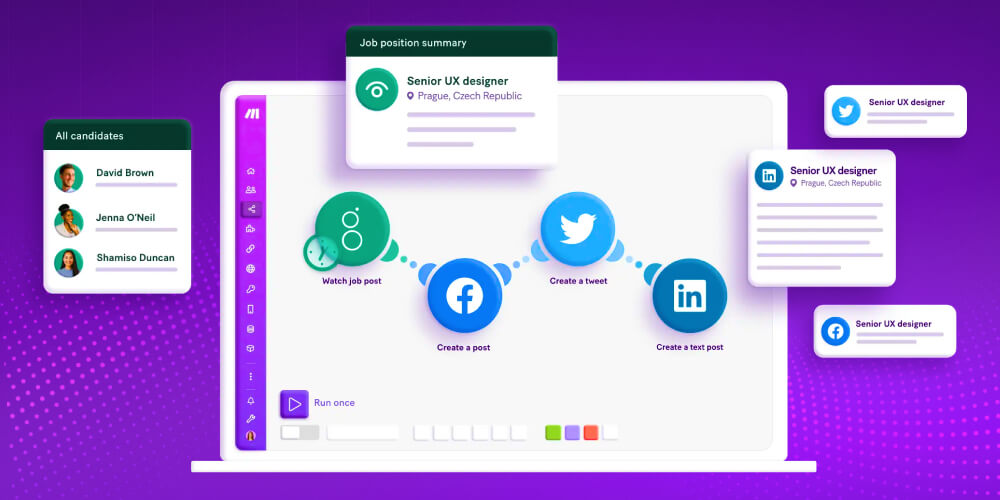
\includegraphics[width=0.8\textwidth]{img/Picture4.png}

    \caption{Make.com}
    \label{fig:make}
\end{figure}

%----------------------------------------------------

\subsection{N8N – nền tảng mã nguồn mở}

\textbf{Định nghĩa:} N8N là nền tảng Automation mã nguồn mở, có thể Self-hosted, đảm bảo bảo mật và tùy biến cao.

\textbf{Thành phần:}
\begin{itemize}
    \item Workflow.
    \item Node.
    \item Trigger Node.
    \item Action Node.
    \item Credential Management.
    \item Database Storage.
    \item Error Workflow.
\end{itemize}

\textbf{Ứng dụng (KingPhone):}
\begin{itemize}
    \item Nhận tin nhắn khách hàng.
    \item Phân loại tin nhắn.
    \item AI phân tích, phản hồi.
    \item Kết nối Sheets/Drive gửi sản phẩm.
    \item Lưu trữ hội thoại.
    \item Quản trị viên kiểm soát.
\end{itemize}

\textbf{Ưu điểm:}
\begin{itemize}
    \item Mã nguồn mở, tự triển khai.
    \item Tùy biến cao.
    \item Chi phí thấp.
    \item Tích hợp AI, API mạnh.
    \item Cộng đồng phát triển năng động.
\end{itemize}

\textbf{Nhược điểm:}
\begin{itemize}
    \item Yêu cầu kiến thức kỹ thuật.
    \item Cần hạ tầng riêng.
    \item Độ phức tạp ban đầu cao.
    \item Hiệu năng phụ thuộc Server.
\end{itemize}

\begin{figure}
\centering
    
\includegraphics[width=0.8\textwidth]{img/Picture5.png}

    \caption{ N8N}
    \label{fig:n8n}
\end{figure}

%----------------------------------------------------

\subsection{WordPress và WooCommerce – nền tảng xây dựng Website thương mại điện tử}

\textbf{Định nghĩa}
WordPress là một hệ quản trị nội dung (CMS – Content Management System) mã nguồn mở, được phát triển từ năm 2003 và hiện là nền tảng Website phổ biến nhất thế giới. Ban đầu WordPress chủ yếu phục vụ viết Blog, nhưng ngày nay đã phát triển thành một nền tảng linh hoạt cho đủ loại Website: tin tức, giáo dục, thương mại điện tử, doanh nghiệp\dots

WooCommerce là một Plugin thương mại điện tử dành cho WordPress, ra mắt năm 2011, cho phép biến Website WordPress thành một cửa hàng trực tuyến đầy đủ chức năng: quản lý sản phẩm, giỏ hàng, thanh toán, đơn hàng, khách hàng. WooCommerce hiện chiếm hơn 25\% các Website thương mại điện tử trên toàn cầu.

\textbf{Thành phần/Cấu trúc}
\begin{itemize}
    \item \textbf{WordPress Core}: Phần lõi mã nguồn mở, cung cấp chức năng quản lý trang, bài viết, người dùng, Media.
    \item \textbf{Theme}: Giao diện Website, có thể tùy chỉnh hoặc cài đặt theme có sẵn để thay đổi thiết kế.
    \item \textbf{Plugin}: Các phần mở rộng bổ sung chức năng, ví dụ: SEO, bảo mật, Livechat, quản lý vận chuyển.
    \item \textbf{WooCommerce}: Plugin cốt lõi để bán hàng, bao gồm:
    \begin{itemize}
        \item Quản lý sản phẩm (thêm, sửa, xóa, phân loại).
        \item Giỏ hàng và thanh toán.
        \item Quản lý đơn hàng, khách hàng.
        \item Tích hợp thanh toán Online, vận chuyển.
    \end{itemize}
    \item \textbf{Database (MySQL/MariaDB)}: Lưu trữ dữ liệu sản phẩm, khách hàng, đơn hàng, cài đặt hệ thống.
\end{itemize}

\textbf{Ứng dụng trong thực tiễn}
Trong đề tài, WordPress + WooCommerce được sử dụng để xây dựng Website bán điện thoại KingPhone:
\begin{itemize}
    \item Hiển thị sản phẩm (IPhone các đời, thông tin, giá bán, hình ảnh).
    \item Cho phép khách hàng thêm sản phẩm vào giỏ, thanh toán trực tuyến.
    \item Quản lý đơn hàng, trạng thái giao dịch.
    \item Tích hợp Plugin SEO (Rank Math SEO) để tối ưu tìm kiếm.
    \item Hỗ trợ Livechat, liên kết với Chatbot Zalo.
    \item Là trung tâm kết nối với hệ thống Make.com.
\end{itemize}


\textbf{Ưu điểm:}
\begin{itemize}
    \item Mã nguồn mở, miễn phí.
    \item Cộng đồng lớn, kho Plugin và Theme phong phú.
    \item Tùy biến linh hoạt, từ Blog nhỏ đến Website lớn.
    \item Thân thiện SEO.
    \item Tích hợp dễ dàng với API, Chatbot, công cụ Automation.
\end{itemize}

\textbf{Nhược điểm:}
\begin{itemize}
    \item Hiệu suất phụ thuộc Plugin.
    \item Bảo mật cần quản lý thường xuyên.
    \item Cần kiến thức kỹ thuật về Server và Database.
    \item Chi phí Hosting cho TMĐT cao hơn so với Blog thông thường.
\end{itemize}

\textbf{Vai trò trong đề tài}
\begin{itemize}
    \item Cửa hàng trực tuyến trung tâm: nơi khách hàng xem và mua điện thoại.
    \item Quản lý đơn hàng, sản phẩm, khách hàng.
    \item Nhận nội dung Marketing tự động từ Make.com.
    \item Kết nối với Chatbot Zalo để hỗ trợ khách hàng.
\end{itemize}

\textbf{Lợi ích:}  
Giúp xây dựng cửa hàng Online chuyên nghiệp, tối ưu quy trình mua bán, và kết hợp với Automation để hình thành một hệ sinh thái số.

Theo số liệu W3Techs 2023, hơn 43\% Website toàn cầu sử dụng WordPress, và WooCommerce là nền tảng thương mại điện tử phổ biến nhất.

\begin{figure}[h!]
    \centering
    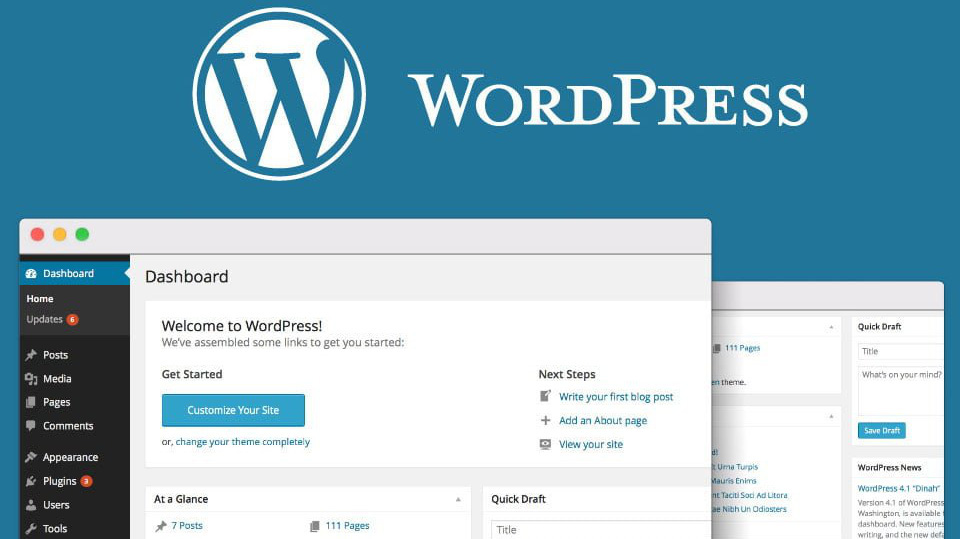
\includegraphics[width=0.75\textwidth]{img/Picture6.png}

    \caption{ Giao diện quản trị WordPress WooCommerce}
    \label{fig:wordpress}
\end{figure}

%---------------------------

\subsection{Facebook Fanpage và YouTube – kênh truyền thông và phân phối nội dung số}

\textbf{Định nghĩa}
\begin{itemize}
    \item \textbf{Facebook Fanpage}: Trang chính thức trên Facebook dành cho doanh nghiệp, thương hiệu hoặc cộng đồng, cho phép đăng tải bài viết, hình ảnh, video, tương tác trực tiếp qua bình luận, tin nhắn.
    \item \textbf{YouTube}: Nền tảng chia sẻ video lớn nhất thế giới, cho phép doanh nghiệp xây dựng kênh chính thức để đăng tải Video giới thiệu sản phẩm, hướng dẫn sử dụng, quảng cáo.
\end{itemize}

\textbf{Thành phần/Cấu trúc}
\textbf{Facebook Fanpage:}
\begin{itemize}
    \item Bài viết (Posts).
    \item Video/Live Stream.
    \item Messenger Chat.
    \item Insight \& Analytics.
\end{itemize}

\textbf{YouTube Channel:}
\begin{itemize}
    \item Video Uploads.
    \item Playlist.
    \item Comment \& Interaction.
    \item YouTube Studio.
\end{itemize}

\textbf{Ứng dụng trong thực tiễn}
\begin{itemize}
    \item Tích hợp Make.com để đăng nội dung tự động.
    \item Fanpage tiếp cận và chăm sóc khách hàng.
    \item YouTube tạo thư viện video marketing dài hạn.
\end{itemize}


\textbf{Ưu điểm:}
\begin{itemize}
    \item Tiếp cận khách hàng lớn.
    \item Đa dạng nội dung: văn bản, hình ảnh, Video, Livestream.
    \item Tăng tương tác, hỗ trợ quảng cáo.
    \item Công cụ phân tích chi tiết.
\end{itemize}

\textbf{Nhược điểm:}
\begin{itemize}
    \item Cạnh tranh cao.
    \item Phụ thuộc thuật toán.
    \item Cần duy trì thường xuyên.
\end{itemize}

\textbf{Vai trò trong đề tài}
\begin{itemize}
    \item \textbf{Facebook Fanpage}: Kênh Marketing chính, đăng tải Video quảng cáo tự động.
    \item \textbf{YouTube}: Kênh truyền thông bổ trợ, lưu trữ Video dài hạn, tăng độ tin cậy thương hiệu.
\end{itemize}

\begin{figure}[h!]
    \centering
    
\includegraphics[width=0.75\textwidth]{img/Picture7.png}
    
    \caption{ Fanpage Facebook và YouTube Channel}
    \label{fig:fb-yt}
\end{figure}

%---------------------------

\subsection{Supabase – nền tảng cơ sở dữ liệu và Backend mã nguồn mở}

\textbf{Định nghĩa}
Supabase là một nền tảng Backend-as-a-Service (BaaS) mã nguồn mở, dựa trên PostgreSQL. Nó cung cấp Real-time database, API tự động sinh, Authentication, Storage và Serverless Functions.
\begin{figure}[h!]
    \centering
    
\includegraphics[width=0.75\textwidth]{img/Picture8.png}
    
    \caption{Supabase}
    \label{fig:supabase}
\end{figure}
\textbf{Thành phần/Cấu trúc}
\begin{itemize}
    \item PostgreSQL Database.
    \item Supabase API (RESTful \& GraphQL).
    \item Authentication.
    \item Realtime.
    \item Storage.
    \item Edge Functions.
    \item Dashboard.
\end{itemize}

\textbf{Ứng dụng trong thực tiễn}
\begin{itemize}
    \item Lưu trữ khách hàng, sản phẩm, đơn hàng.
    \item Đồng bộ dữ liệu Real-time.
    \item Quản lý xác thực người dùng.
    \item Lưu file (ảnh, Video).
    \item Xử lý nghiệp vụ bằng Edge Functions.
\end{itemize}


\textbf{Ưu điểm:} Mã nguồn mở, API tự động, Realtime mạnh, bảo mật cao, chi phí hợp lý. 

\textbf{Nhược điểm:} Đang phát triển, cần kiến thức PostgreSQL, hiệu năng phụ thuộc hạ tầng, cộng đồng nhỏ hơn Firebase.

\textbf{Vai trò trong đề tài}
\begin{itemize}
    \item Thay thế/bổ sung Google Sheets/Drive.
    \item Lưu trữ dữ liệu sản phẩm, khách hàng.
    \item Quản lý xác thực.
    \item Tích hợp N8N/Make.com qua API.
\end{itemize}



%---------------------------

\subsection{PostgreSQL – hệ quản trị cơ sở dữ liệu quan hệ mã nguồn mở}

\textbf{Định nghĩa}
PostgreSQL (Postgres) là hệ quản trị cơ sở dữ liệu quan hệ (RDBMS) mã nguồn mở, phát triển từ 1986 tại Đại học California, Berkeley. Nó nổi bật nhờ khả năng lưu trữ dữ liệu quan hệ, hỗ trợ JSON, XML, GIS\dots

\begin{figure}[h!]
    \centering
    
\includegraphics[width=0.65\textwidth]{img/Picture9.png}
    
    \caption{ PostgreSQL}
    \label{fig:postgresSLQ}
\end{figure}

\textbf{Thành phần/Cấu trúc}
\begin{itemize}
    \item Database Cluster.
    \item Database.
    \item Schema.
    \item Table.
    \item Data Types.
    \item Query Engine.
    \item Index.
    \item Transaction \& ACID.
    \item Replication.
\end{itemize}

\textbf{Ứng dụng trong thực tiễn}
\begin{itemize}
    \item Web và ứng dụng TMĐT.
    \item Chatbot \& Automation.
    \item Phân tích dữ liệu.
    \item GIS với PostGIS.
    \item Backend hiện đại (Supabase, Hasura).
\end{itemize}

\textbf{Ưu điểm:} Mã nguồn mở, chuẩn SQL, mở rộng mạnh, ổn định và bảo mật, replication tốt. 

\textbf{Nhược điểm:} Cần kỹ năng quản trị, hiệu năng thấp hơn NoSQL ở dữ liệu phi cấu trúc, khó tối ưu Big Data.

\textbf{Vai trò trong đề tài}
\begin{itemize}
    \item Lưu trữ dữ liệu sản phẩm, khách hàng, đơn hàng.
    \item Hỗ trợ Chatbot và Website.
    \item Thay thế Google Sheets khi cần Database chuyên nghiệp.
    
\end{itemize}

\\
\section{KẾT QUẢ NGHIÊN CỨU TRONG VÀ NGOÀI NƯỚC CÓ LIÊN QUAN}
\subsection{Kết quả nghiên cứu trong nước}
Tại Việt Nam, nhiều nghiên cứu tập trung vào việc áp dụng Chatbot trong các lĩnh vực thương mại điện tử, giáo dục, và dịch vụ công. Các đề tài này nhấn mạnh khả năng:
\begin{itemize}
    \item Hỗ trợ tự động tư vấn khách hàng, tiết kiệm thời gian và chi phí nhân sự.
    \item Ứng dụng Chatbot trong quảng bá sản phẩm, bán hàng trực tuyến.
    \item Nâng cao trải nghiệm khách hàng nhờ phản hồi nhanh chóng và chính xác.
\end{itemize}

Các nghiên cứu thực nghiệm cũng cho thấy việc ứng dụng Chatbot Zalo có tiềm năng lớn vì đây là nền tảng có số lượng người dùng cao tại Việt Nam, phù hợp cho doanh nghiệp vừa và nhỏ.

\subsection{Kết quả nghiên cứu ngoài nước}
Trên thế giới, nhiều công trình khoa học đã khẳng định hiệu quả của Chatbot trong thương mại điện tử và marketing số. Một số xu hướng nổi bật:
\begin{itemize}
    \item Chatbot ứng dụng trí tuệ nhân tạo (AI) và xử lý ngôn ngữ tự nhiên (NLP) để hiểu ngữ cảnh và cải thiện độ chính xác khi giao tiếp.
    \item Kết hợp Chatbot với hệ thống quản lý khách hàng (CRM) giúp cá nhân hóa dịch vụ.
    \item Ứng dụng Chatbot trong đa dạng lĩnh vực như chăm sóc y tế, tài chính, giáo dục và thương mại.
\end{itemize}

Các nghiên cứu ngoài nước cũng chỉ ra rằng Chatbot không chỉ dừng ở việc trả lời tự động, mà còn là công cụ thu thập dữ liệu, phân tích hành vi khách hàng và đưa ra gợi ý sản phẩm phù hợp. Điều này mở ra triển vọng lớn cho các doanh nghiệp trong việc tối ưu hóa chiến lược kinh doanh.



\chapter{KẾT QUẢ - THẢO LUẬN}

\section{Nội dung thực hiện TTTN}

Trong quá trình thực tập tại doanh nghiệp, tôi đã có cơ hội tham gia trực tiếp vào
các hoạt động liên quan đến việc nghiên cứu, thiết kế và triển khai hệ thống tự động
hóa truyền thông và thương mại điện tử thông qua nền tảng Chatbot Zalo. Nội dung
thực hiện được chia thành ba phần chính: tìm hiểu quy trình làm việc tại doanh nghiệp,
nắm bắt nội dung đề tài, và trực tiếp tham gia các công việc cụ thể trong quá trình
thực tập.

\subsection*{Tổng quan về quy trình làm việc tại doanh nghiệp}
Doanh nghiệp nơi tôi thực tập hoạt động chủ yếu trong lĩnh vực kinh doanh truyền thống. Quy trình làm việc cơ bản bao gồm các giai đoạn: tiếp cận khách
hàng, giới thiệu sản phẩm, hỗ trợ khách hàng, tiếp nhận và xử lý đơn hàng, chăm sóc
khách hàng sau bán. Hiện tại, các công việc này được thực hiện song song trên nhiều
nền tảng như Website, Facebook và đặc biệt là Zalo – nơi tập trung một lượng lớn
khách hàng Việt Nam.

Tuy nhiên, phương pháp làm việc truyền thống còn tồn tại nhiều hạn chế: việc
trả lời tin nhắn chủ yếu dựa vào nhân sự chăm sóc khách hàng; các hoạt động quảng bá
sản phẩm chưa đồng bộ; việc quản lý thông tin khách hàng còn rời rạc. Chính vì vậy,
doanh nghiệp mong muốn triển khai một hệ thống tự động hóa có thể giảm thiểu khối
lượng công việc thủ công, đồng thời tăng tính chuyên nghiệp và hiệu quả.

\subsection*{Tổng quan về đề tài thực tập}
Đề tài mà tôi được giao là “Hệ thống Tự động hóa Truyền thông và Thương mại
Điện tử cho Doanh nghiệp ứng dụng Chatbot Zalo”. Đây là một đề tài mang tính ứng
dụng cao, phù hợp với bối cảnh chuyển đổi số hiện nay. Nội dung tập trung vào việc:

\begin{itemize}
    \item Xây dựng hệ thống Chatbot Zalo nhằm hỗ trợ khách hàng tự động, 24/7.
    \item Tích hợp các chức năng giới thiệu sản phẩm, tư vấn, đặt hàng cơ bản.
    \item Quản lý thông tin khách hàng và đơn hàng một cách tập trung.
    \item Kết nối với các công cụ marketing để tăng hiệu quả quảng bá.
\end{itemize}

\subsection*{Quá trình thực hiện công việc}

\begin{itemize}
    \item \textbf{Khảo sát hiện trạng:} Tìm hiểu cách doanh nghiệp đang quản lý
    hoạt động truyền thông và bán hàng. Ghi nhận những khó khăn thường gặp
    như phản hồi chậm, sai sót khi nhập đơn hàng, hay khó khăn trong việc thống
    kê số liệu.

    \item \textbf{Nghiên cứu công nghệ:} Tìm hiểu về nền tảng Zalo API do Zalo cung cấp, cũng như các công cụ hỗ trợ triển khai
    Chatbot như N8N, Make.com.

    \item \textbf{Thiết kế hệ thống:} Đề xuất sơ đồ kiến trúc của hệ thống Chatbot,
    bao gồm: Module giao tiếp với người dùng, Module xử lý ngôn ngữ tự nhiên,
    Module quản lý cơ sở dữ liệu và Module kết nối Marketing.

    \item \textbf{Xây dựng Chatbot cơ bản:} Thiết kế các kịch bản hội thoại, ví dụ:
    chào hỏi khách hàng, cung cấp thông tin sản phẩm, tiếp nhận đơn hàng.

    \item \textbf{Triển khai tính năng mở rộng:} Tích hợp công cụ Marketing để gửi
    tin nhắn chăm sóc định kỳ, tự động phân loại khách hàng tiềm năng, và ghi
    nhận phản hồi.

\end{itemize}

Kết quả bước đầu cho thấy hệ thống Chatbot đã giảm tải đáng kể khối lượng công
việc thủ công của bộ phận chăm sóc khách hàng, đồng thời tạo trải nghiệm mới mẻ và
tiện lợi cho khách hàng.


\section{Phân tích, đánh giá đề tài thực tập}

\subsection*{Hiệu quả đạt được}
\begin{itemize}
    \item \textbf{Tiết kiệm thời gian và nhân lực:} Hệ thống Chatbot có khả năng
    trả lời tức thì các câu hỏi cơ bản, chiếm khoảng 70\% khối lượng công việc
    của bộ phận chăm sóc khách hàng. Nhờ vậy, nhân viên có thể tập trung vào
    các tình huống phức tạp hơn.

    \item \textbf{Nâng cao trải nghiệm khách hàng:} Khách hàng có thể tiếp cận
    thông tin sản phẩm nhanh chóng, đặt hàng ngay trên Zalo, và nhận phản hồi
    tức thì. Điều này làm tăng mức độ hài lòng và sự gắn kết.

    \item \textbf{Quản lý dữ liệu tập trung:} Thông tin khách hàng, đơn hàng và
    lịch sử tương tác được lưu trữ trên một hệ thống thống nhất, giúp việc phân
    tích hành vi và lên kế hoạch marketing hiệu quả hơn.

    \item \textbf{Hỗ trợ Marketing:} Hệ thống cho phép gửi tin nhắn định kỳ,
    khuyến mãi và thông báo đến từng nhóm khách hàng mục tiêu, từ đó gia tăng
    tỷ lệ chuyển đổi.
\end{itemize}

\section{Giải pháp}

\subsection{Chuẩn hóa tài liệu \& tri thức vận hành (Ưu tiên rất cao)}
\textbf{Vấn đề:} Thiếu tài liệu chi tiết.  

\textbf{Giải pháp:} Xây dựng bộ tài liệu chuẩn hóa (kiến trúc hệ thống, hướng dẫn cài đặt, giải thích workflow, xử lý sự cố).  

\textbf{Lợi ích:} Rút ngắn đào tạo, giảm rủi ro vận hành.  

\subsection{Đào tạo trọng điểm (Ưu tiên cao)}
\textbf{Vấn đề:} Đội ngũ thiếu kỹ năng chuyên sâu. 

\textbf{Giải pháp:} Workshop Flutter/Dart, N8N, Make.com, WordPress, Prompt Engineering, bảo mật API.  

\textbf{Lợi ích:} Nâng cao năng lực, tăng tốc triển khai.  

\subsection{Tối ưu hiệu năng \& trải nghiệm người dùng (Ưu tiên cao)}
\textbf{Vấn đề:} Độ trễ chatbot, tốc độ tải web chưa tối ưu.  

\textbf{Giải pháp:} Cache chatbot, nén ảnh, CDN, batch xử lý Make.com. 

\textbf{Lợi ích:} Mượt mà, tăng hài lòng khách hàng.  

\subsection{Tăng cường an toàn \& bảo mật (Ưu tiên cao)}
\textbf{Vấn đề:} Nguy cơ rò rỉ dữ liệu.  

\textbf{Giải pháp:} Supabase Auth, Security Rules, mã hóa token, Secret Manager.  

\textbf{Lợi ích:} Bảo vệ dữ liệu, giảm rủi ro tấn công.  

\subsection{Mở rộng dữ liệu sang Supabase/PostgreSQL (Ưu tiên TB → Cao)}
\textbf{Vấn đề:} Google Sheets hạn chế dữ liệu lớn.  

\textbf{Giải pháp:} Di chuyển core data sang PostgreSQL, Sheets chỉ dùng nhập liệu nhanh.  

\textbf{Lợi ích:} Mở rộng, xử lý hàng nghìn sản phẩm.  

\subsection{Tìm kiếm \& đề xuất thông minh (Ưu tiên TB)}
\textbf{Vấn đề:} Tìm kiếm/đề xuất sản phẩm hạn chế.  

\textbf{Giải pháp:} Tích hợp Algolia/Elasticsearch, AI Recommendation. 

\textbf{Lợi ích:} Nâng cao trải nghiệm, tăng chuyển đổi.  

\subsection{Giám sát, đo lường \& tối ưu chi phí (Ưu tiên TB)}
\textbf{Vấn đề:} Thiếu giám sát hiệu năng/chi phí. 

\textbf{Giải pháp:} Grafana/Metabase, đo chi phí API, cảnh báo sự cố.  

\textbf{Lợi ích:} Chủ động xử lý sự cố, tối ưu chi phí.  

\subsection{Nâng cấp chức năng kinh doanh cốt lõi (Ưu tiên TB)}
\textbf{Vấn đề:} Thiếu tính năng TMĐT hiện đại.  


\textbf{Giải pháp:} Thanh toán online, quản lý kho, AI khuyến mãi.  
\textbf{Lợi ích:} Nền tảng TMĐT chuyên nghiệp, tăng doanh thu.  

\subsection{Kiểm thử toàn diện \& đa thiết bị (Ưu tiên TB)}
\textbf{Vấn đề:} Chưa kiểm thử đủ tình huống.  

\textbf{Giải pháp:} Firebase Test Lab, thiết bị thật, load test.

\textbf{Lợi ích:} Ổn định, sẵn sàng cho nhiều khách hàng.  

\subsection{Quản trị nội dung \& thương hiệu bằng AI có kiểm soát (Ưu tiên TB)}
\textbf{Vấn đề:} Nội dung AI thiếu kiểm soát giọng thương hiệu.

\textbf{Giải pháp:} Workflow phê duyệt, Prompt chuẩn hóa. 

\textbf{Lợi ích:} Nội dung nhất quán, tối ưu sáng tạo.
\section{WORKFLOW hệ thống và WORDPRESS}

\subsection{Workflow hệ thống}


\subsubsection{Workflow tự động truyền thông đa kênh Make.com}

\begin{figure}[h!]
    \centering
    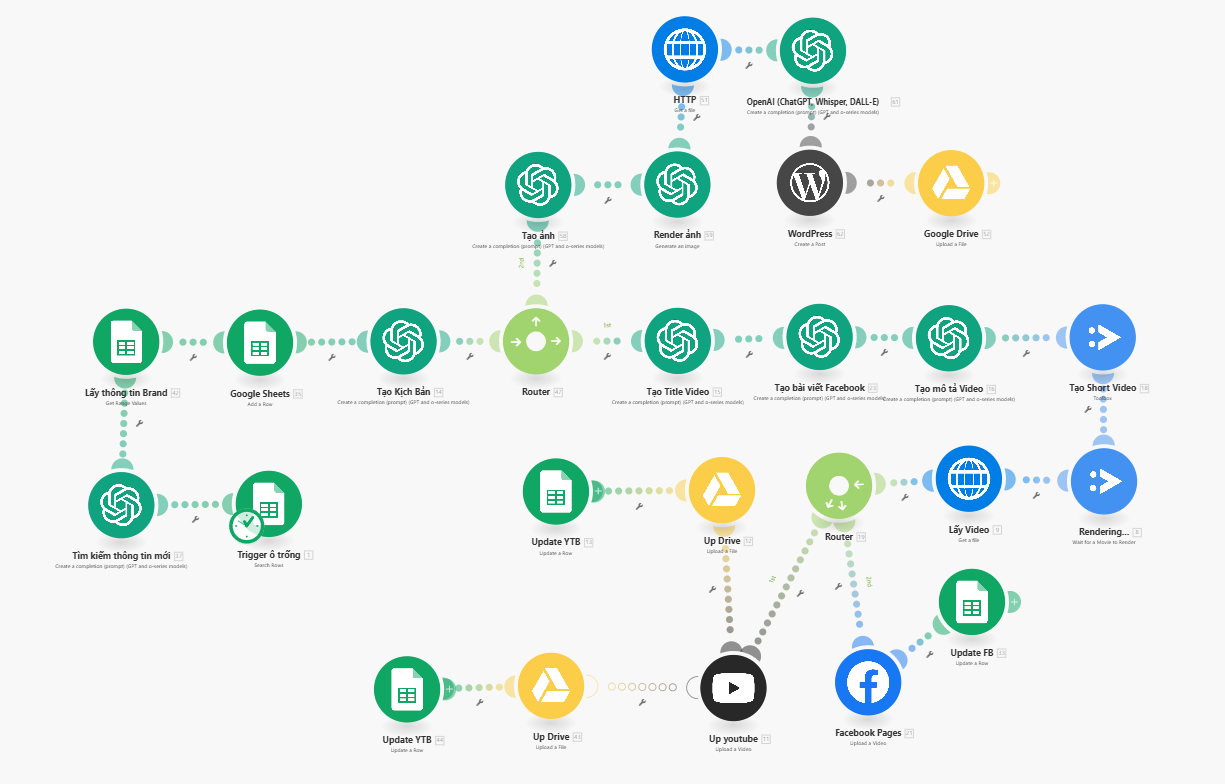
\includegraphics[width=0.6\textwidth]{img/Picture10.png}
    \caption{Workflow truyền thông đa kênh Make.com}
    \label{fig:workflow-make}
\end{figure}

\subsubsection{Workflow tự động tạo nội dung và Video truyền thông đa kênh}

\begin{figure}[h!]
    \centering
    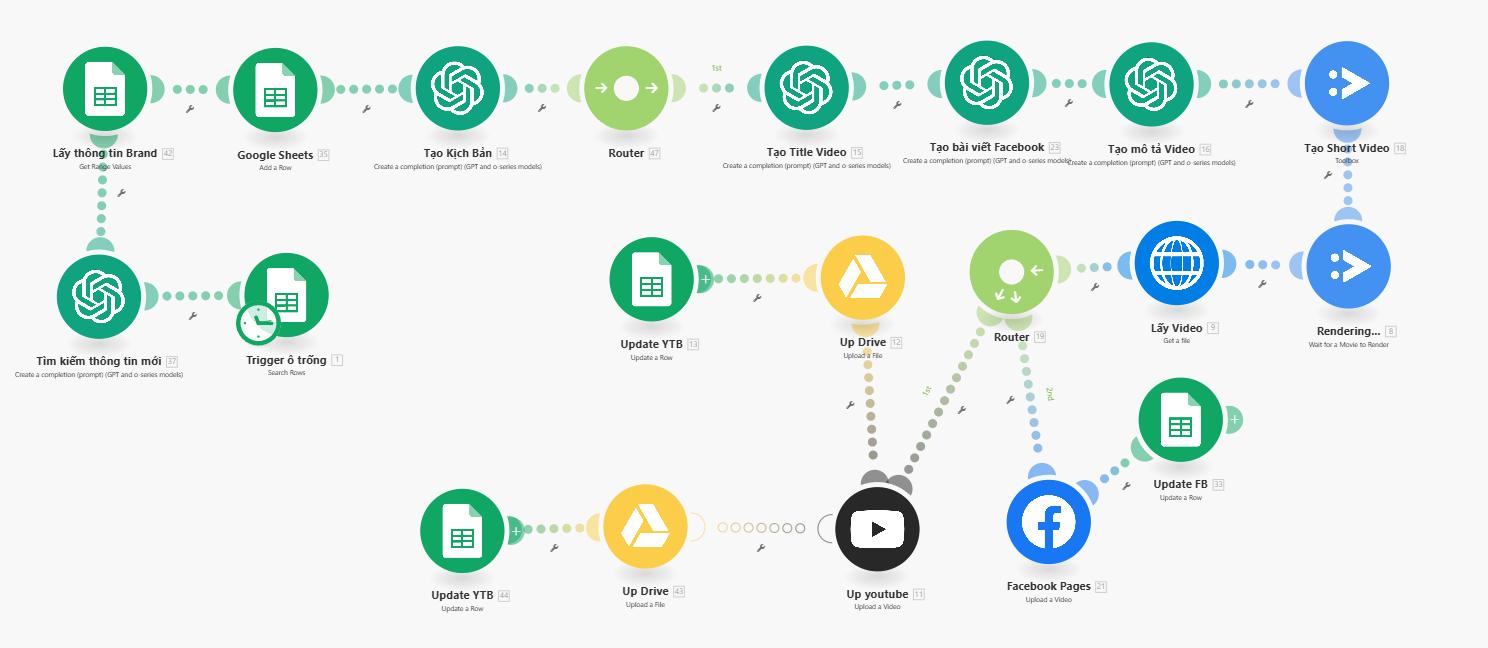
\includegraphics[width=0.6\textwidth]{img/Picture11.png}
    \caption{Workflow tự động tạo nội dung và Video truyền thông đa kênh}
    \label{fig:workflow-video}
\end{figure}

\subsubsection{Workflow tự động tạo bài viết và hình truyền thông Wordpress}

\begin{figure}[h!]
    \centering
    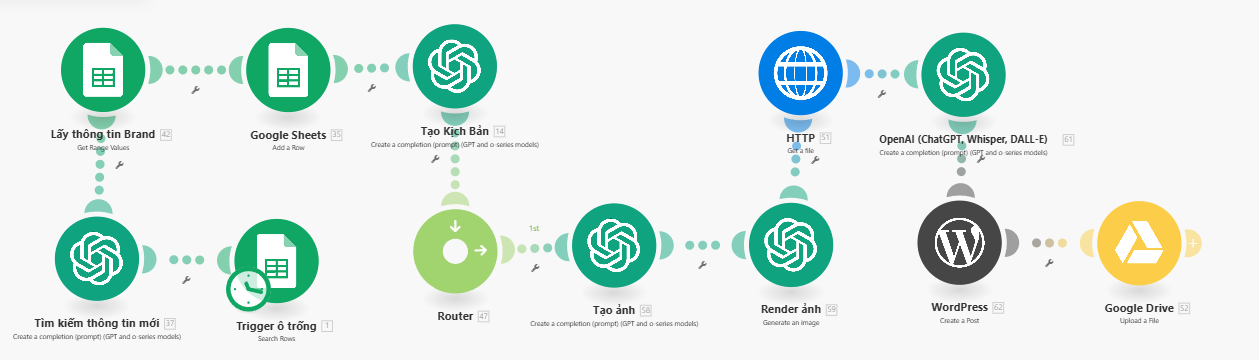
\includegraphics[width=0.6\textwidth]{img/Picture12.png}
    \caption{Workflow tự động tạo bài viết và hình truyền thông Wordpress}
    \label{fig:workflow-wordpress}
\end{figure}

\subsubsection{Kết quả Workflow tự động truyền thông đa kênh}

\begin{figure}[H]
    \centering
    
\includegraphics[width=0.6\textwidth]{img/Picture13.png}
    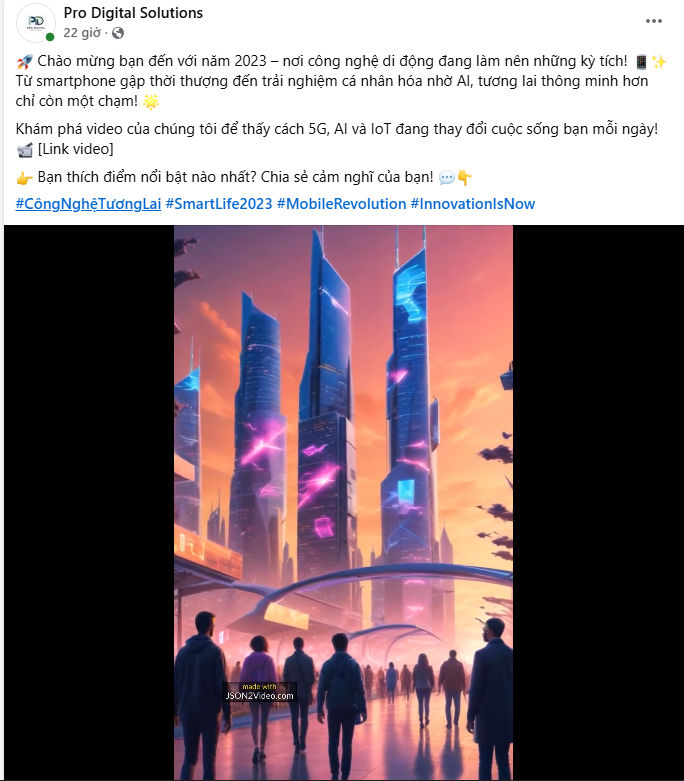
\includegraphics[width=0.6\textwidth]{img/Picture14.png}
    \caption{Kết quả Workflow tự động truyền thông đa kênh}
    \label{fig:workflow-ketqua}
\end{figure}

\subsubsection{Workflow Chatbot Zalo phân loại và trả lời tin nhắn}

\begin{figure}[H]
    \centering
    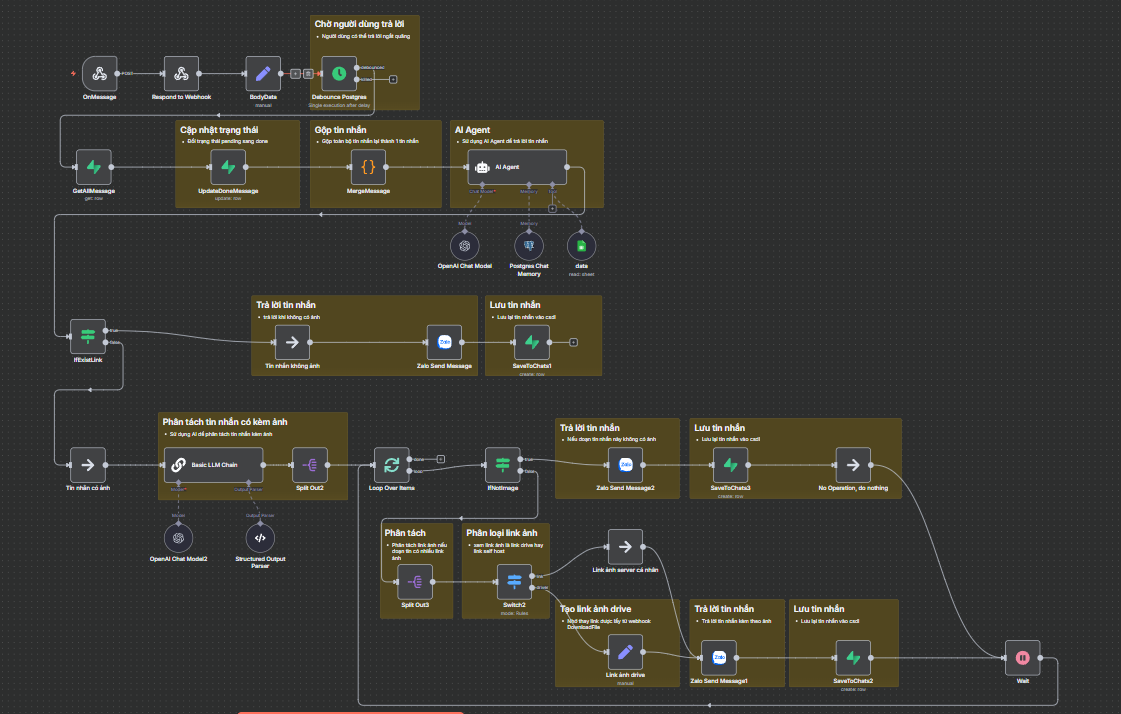
\includegraphics[width=0.6\textwidth]{img/Picture15.png}
    \caption{Workflow chatbot Zalo phân loại và trả lời tin nhắn}
    \label{fig:chatbot-phanloai}
\end{figure}

\subsubsection{Workflow chatbot Zalo tiếp nhận tin nhắn, phân loại và lưu trữ}

\begin{figure}[H]
    \centering
    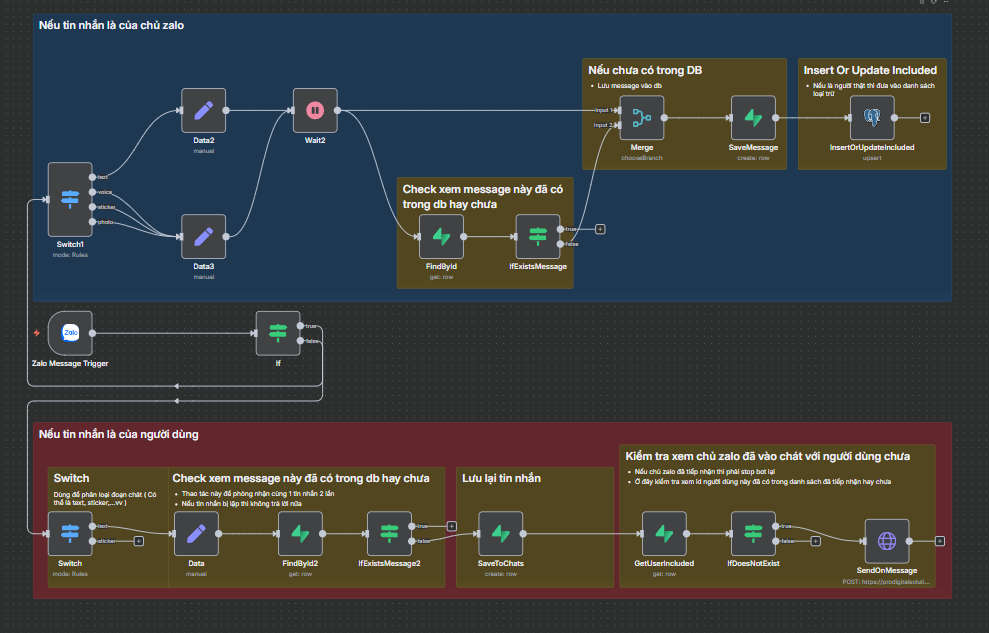
\includegraphics[width=0.6\textwidth]{img/Picture16.png}
    \caption{Workflow chatbot Zalo tiếp nhận tin nhắn, phân loại và lưu trữ}
    \label{fig:chatbot-luutru}
\end{figure}

\subsubsection{Workflow tải hình ảnh từ Google Drive và khởi tạo cơ sở dữ liệu}

\begin{figure}[H]
    \centering
    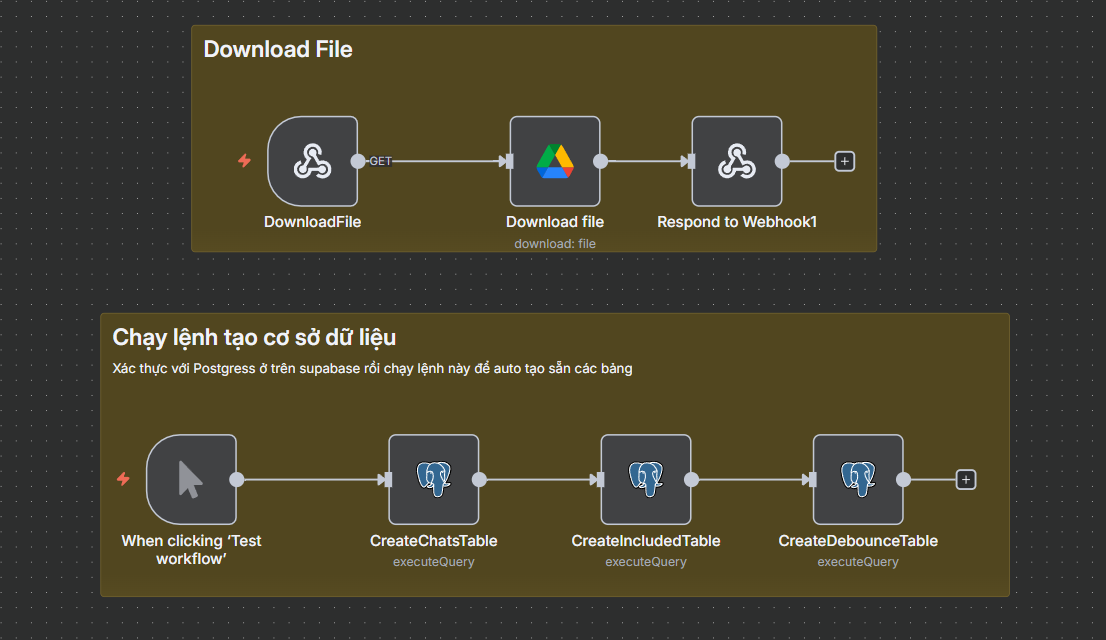
\includegraphics[width=0.6\textwidth]{img/Picture17.png}
    \caption{Workflow tải hình ảnh từ Google Drive và khởi tạo cơ sở dữ liệu}
    \label{fig:chatbot-drive}
\end{figure}



\subsubsection{Kết quả Chatbot Zalo hỗ trợ tư vấn khách hàng}
\begin{figure}[H]
    \centering
    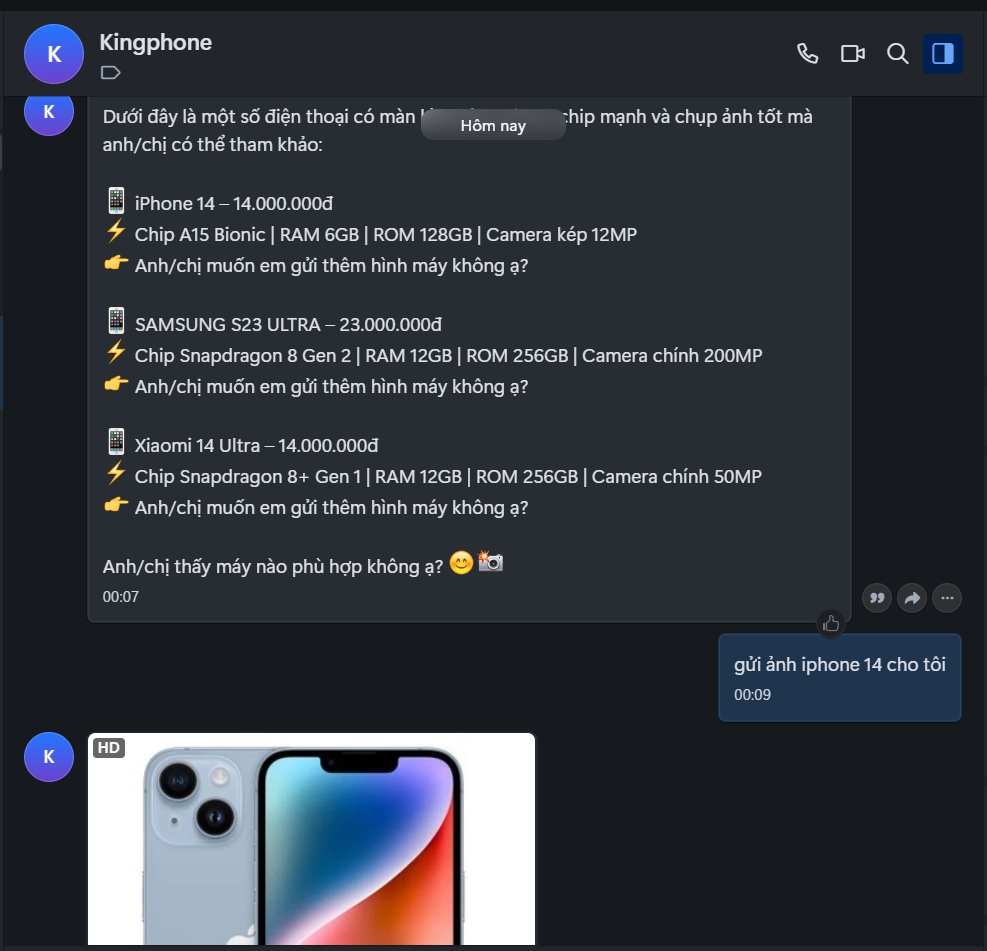
\includegraphics[width=0.6\textwidth]{img/Picture18.png}
    \caption{Kết quả Chatbot Zalo hỗ trợ tư vấn khách hàng}
    \label{fig:chatbot-ketqua1}
    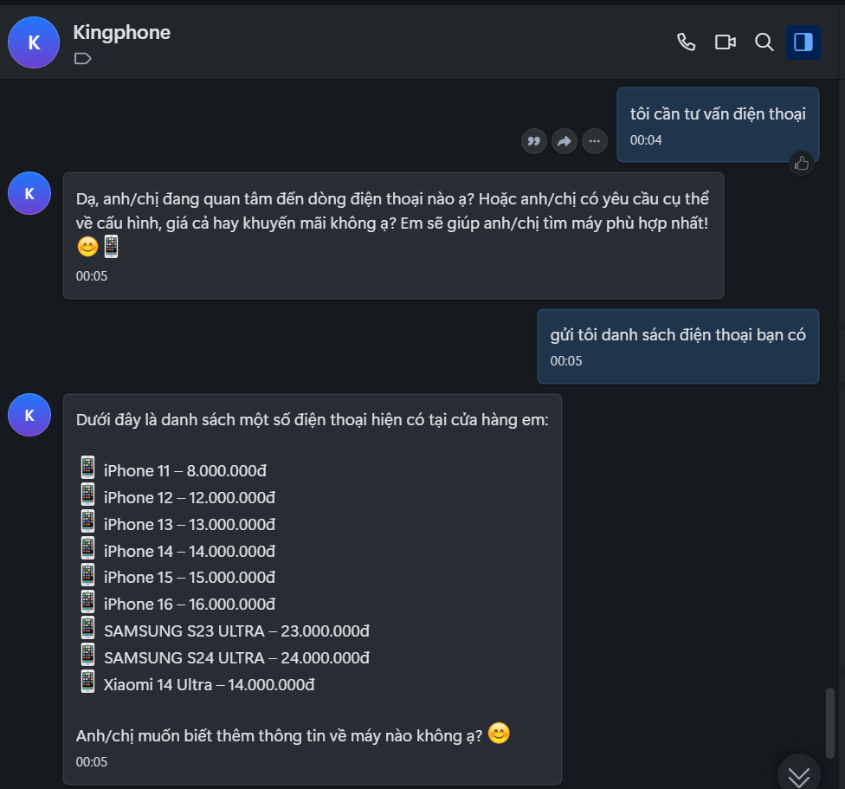
\includegraphics[width=0.6\textwidth]{img/Picture19.png}
    \caption{Kết quả Chatbot Zalo hỗ trợ tư vấn khách hàng}
    \label{fig:chatbot-ketqua}
\end{figure}
\subsection{Wordpress}

\subsubsection{Trang chủ}
\begin{figure}[H]
    \centering
    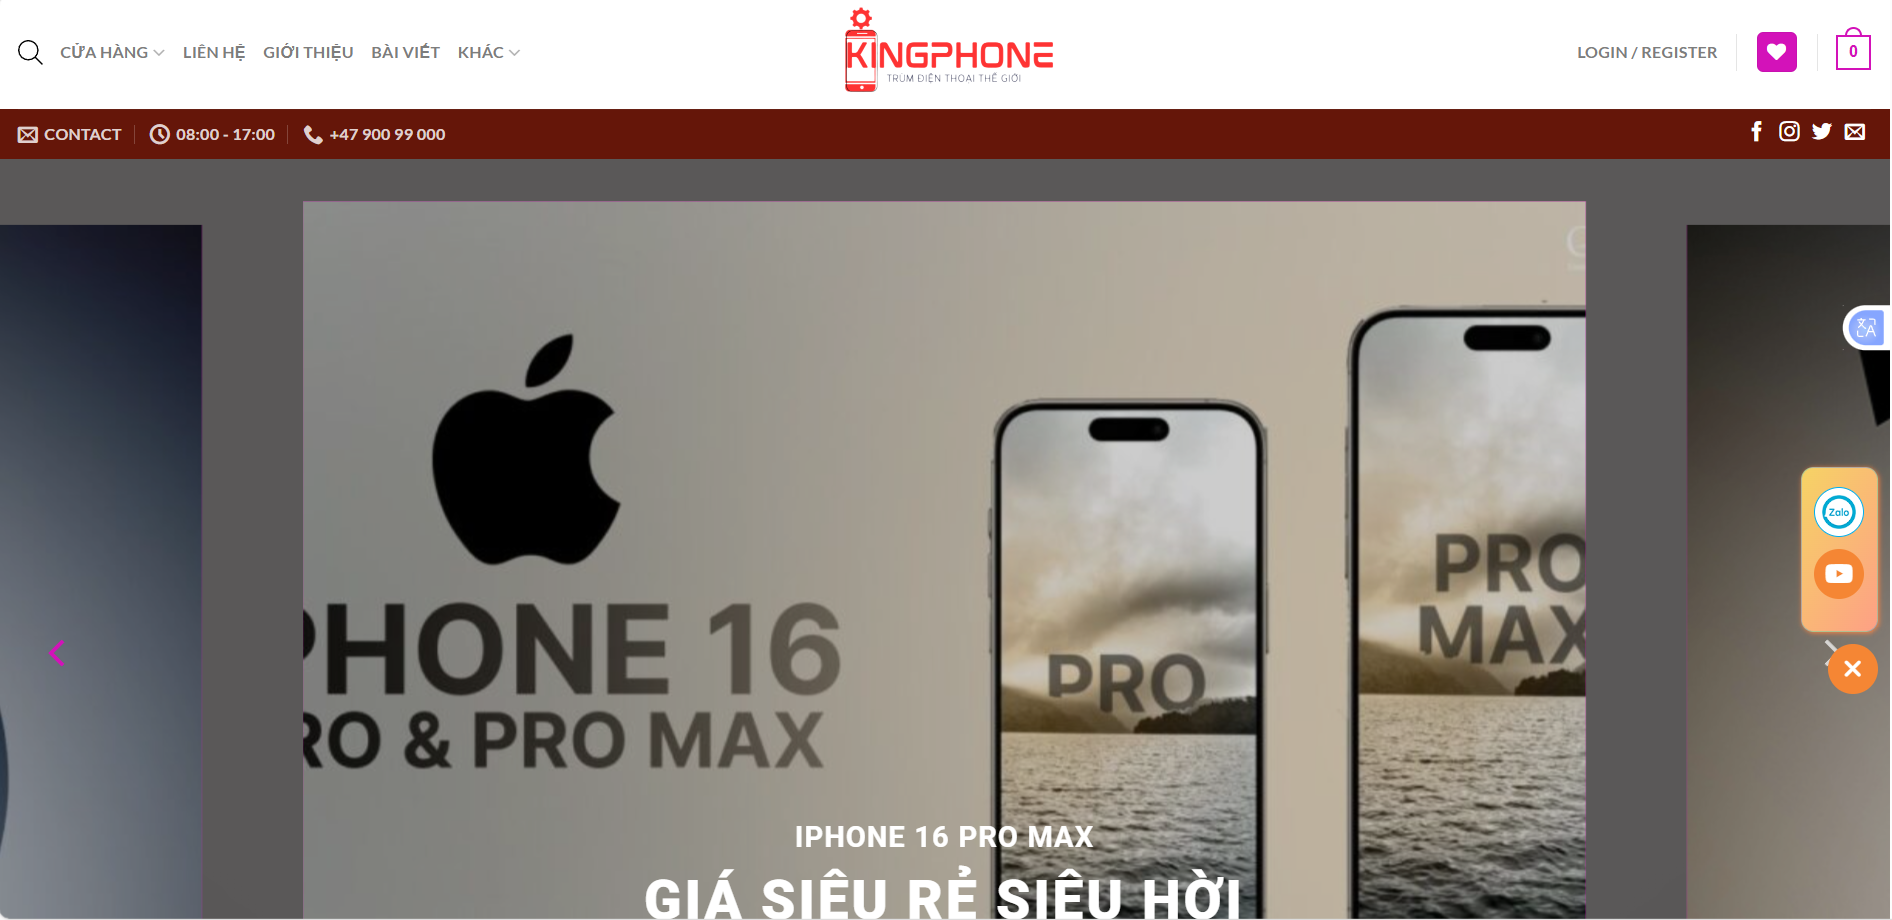
\includegraphics[width=0.6\textwidth]{img/trangchu1.png}
    \caption{Trang chủ 1}
    \label{fig:tc}
\end{figure}
\subsubsection{Header}
\begin{figure}[H]
    \centering
    
\includegraphics[width=0.6\textwidth]{img/header.png}
    \caption{Trang Header}
    \label{fig:header}
\end{figure}
\subsubsection{Footer}
\begin{figure}[H]
    \centering
    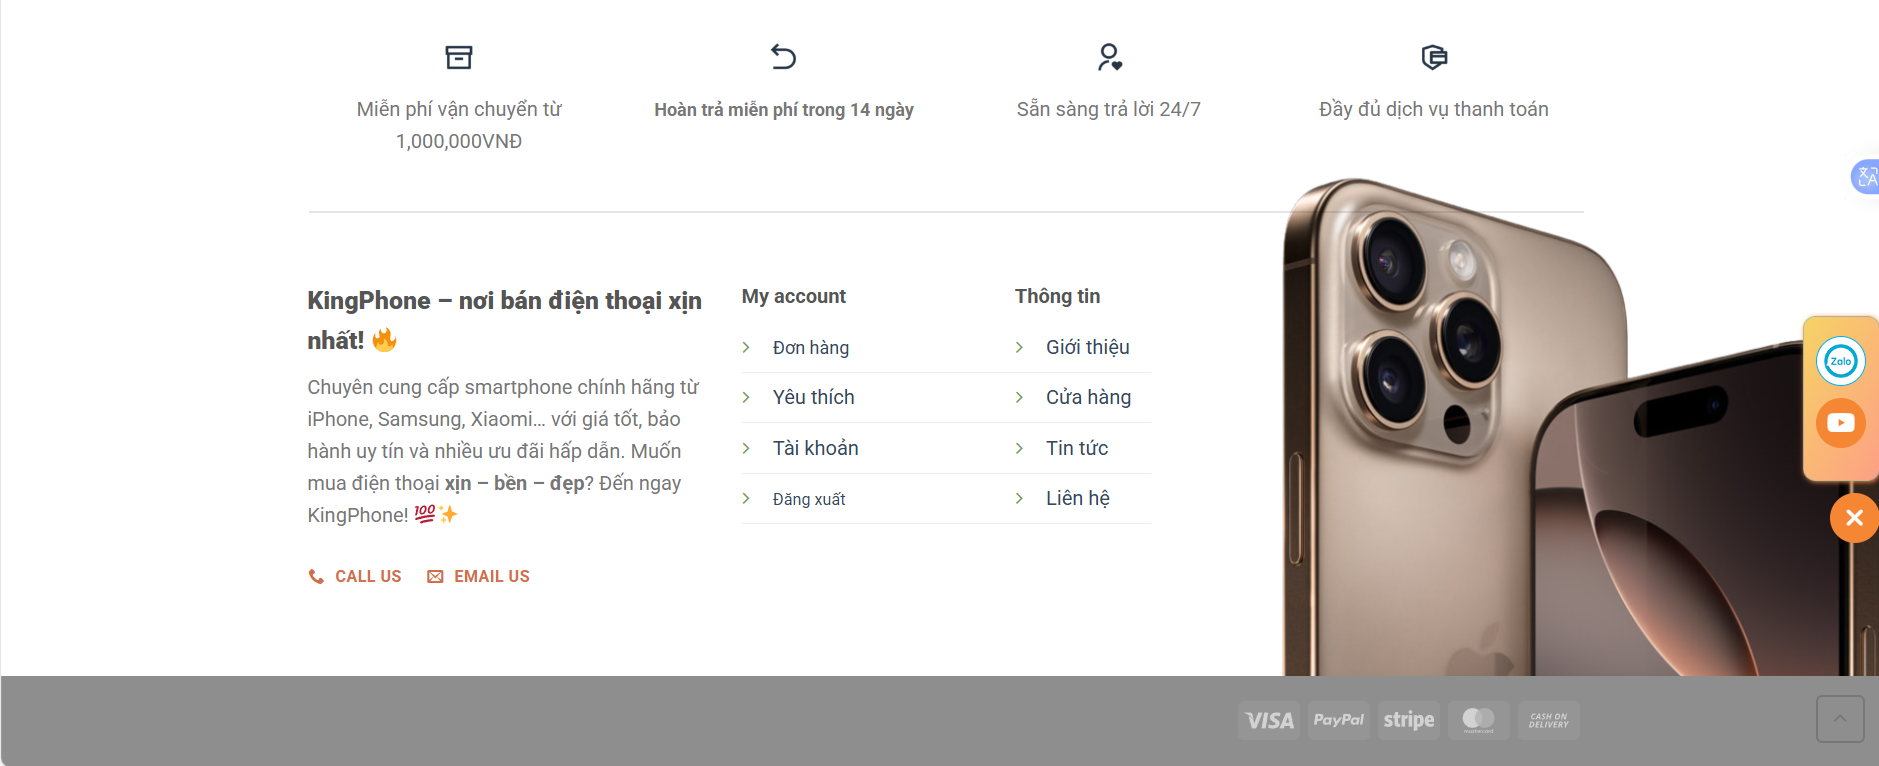
\includegraphics[width=0.6\textwidth]{img/footer.png}
    \caption{Trang Footer}
    \label{fig:foter}
\end{figure}
\subsubsection{Trang Đăng ký/ Đăng nhập}
\begin{figure}[H]
    \centering
    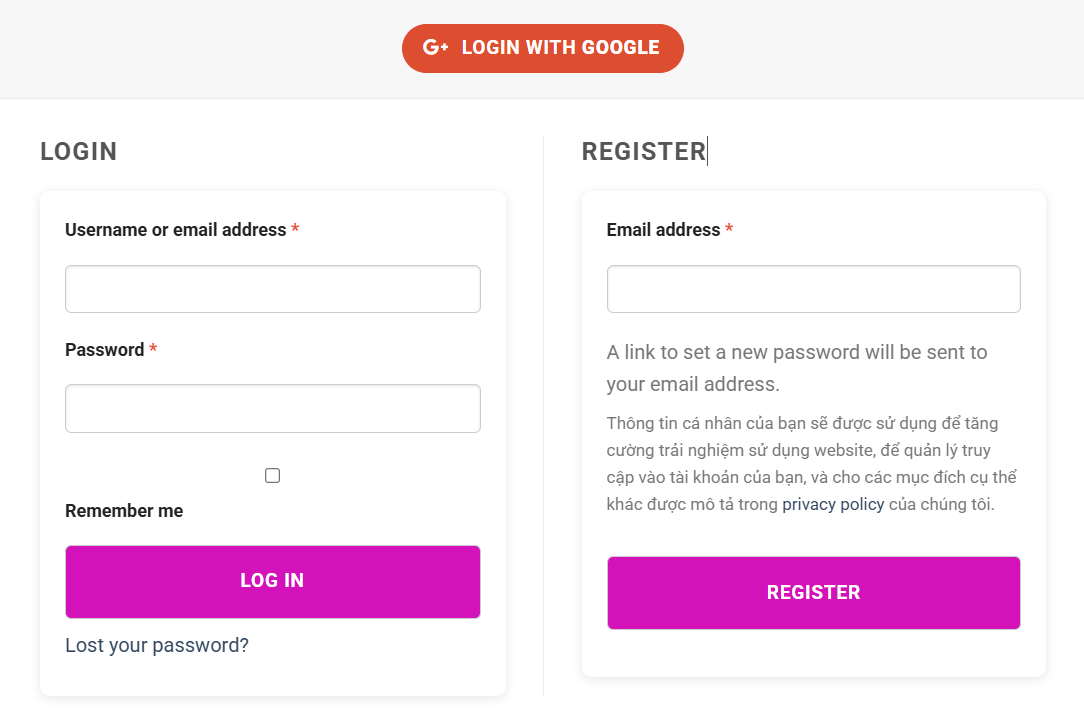
\includegraphics[width=0.6\textwidth]{img/dangnhap.png}
    \caption{Trang đăng ký/đăng nhập}
    \label{fig:dkdn}
\end{figure}

\subsubsection{Trang sản phẩm}
\begin{figure}[H]
    \centering
    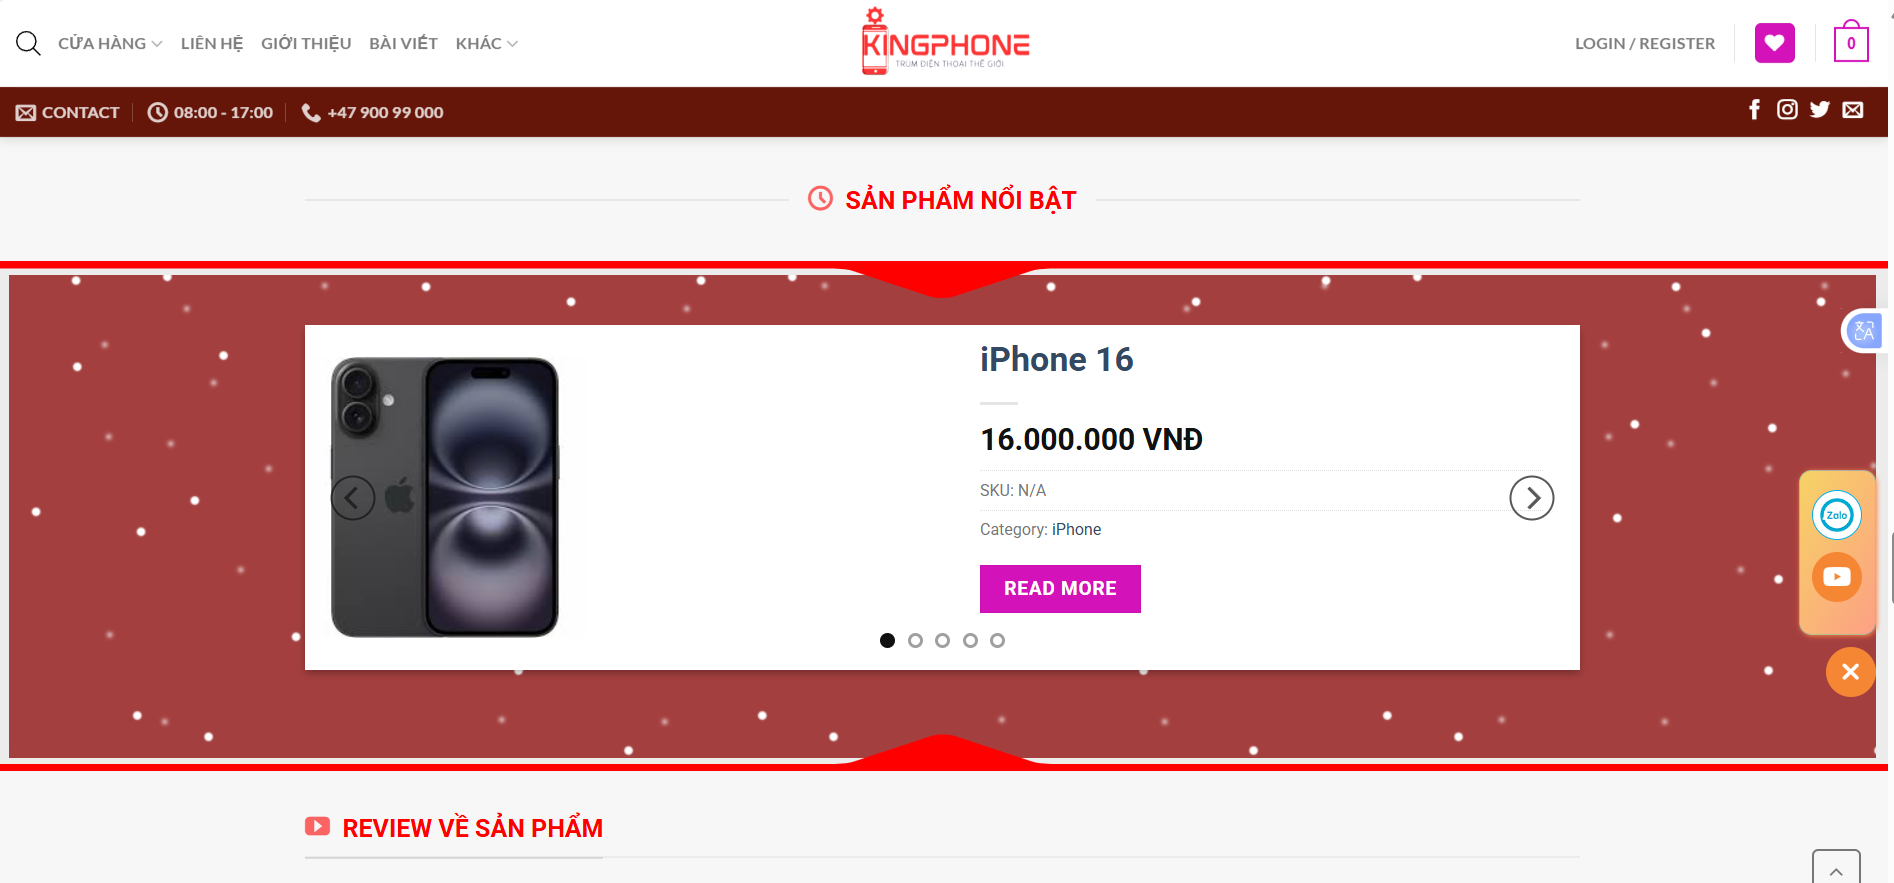
\includegraphics[width=0.6\textwidth]{img/sanpahmnoibat.png}
    \caption{Trang sản phẩm nổi bật}
    \label{fig:noibat}
\end{figure}

\subsubsection{Trang sản phẩm}
\begin{figure}[H]
    \centering
    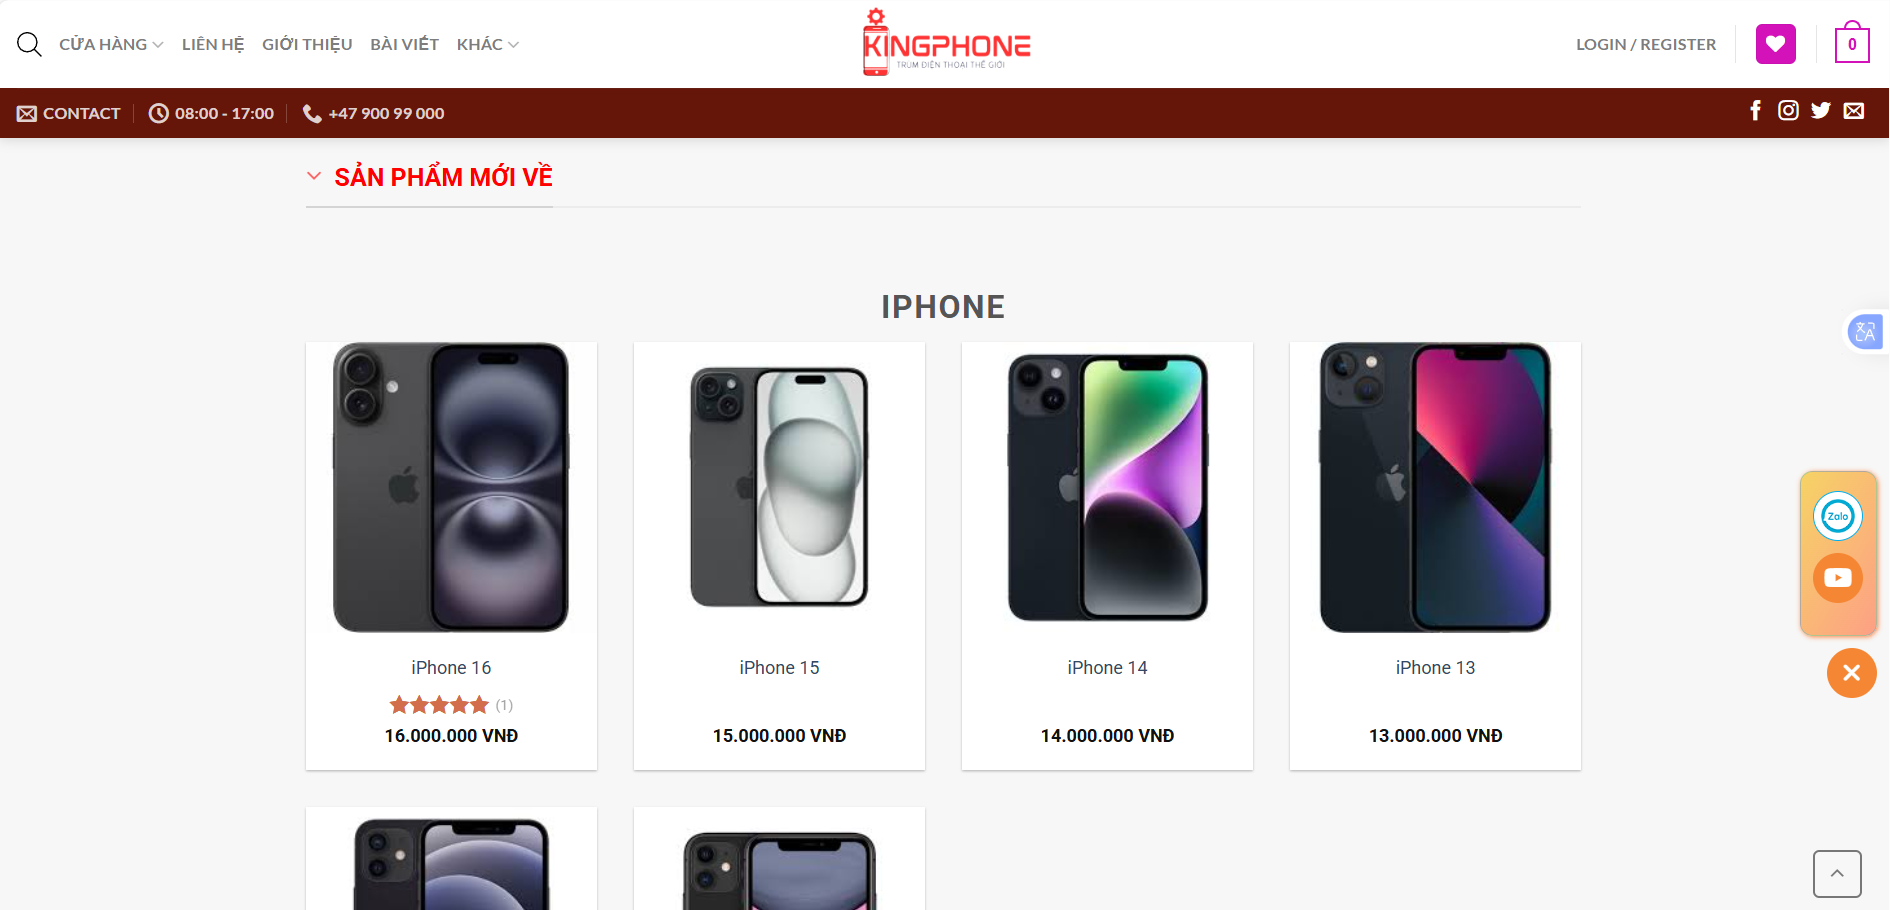
\includegraphics[width=0.6\textwidth]{img/sanphammoive.png}
    \caption{Trang sản phẩm mới về}
    \label{fig:moive}
\end{figure}


\subsubsection{Trang Reviews sản phẩm}
\begin{figure}[H]
    \centering
    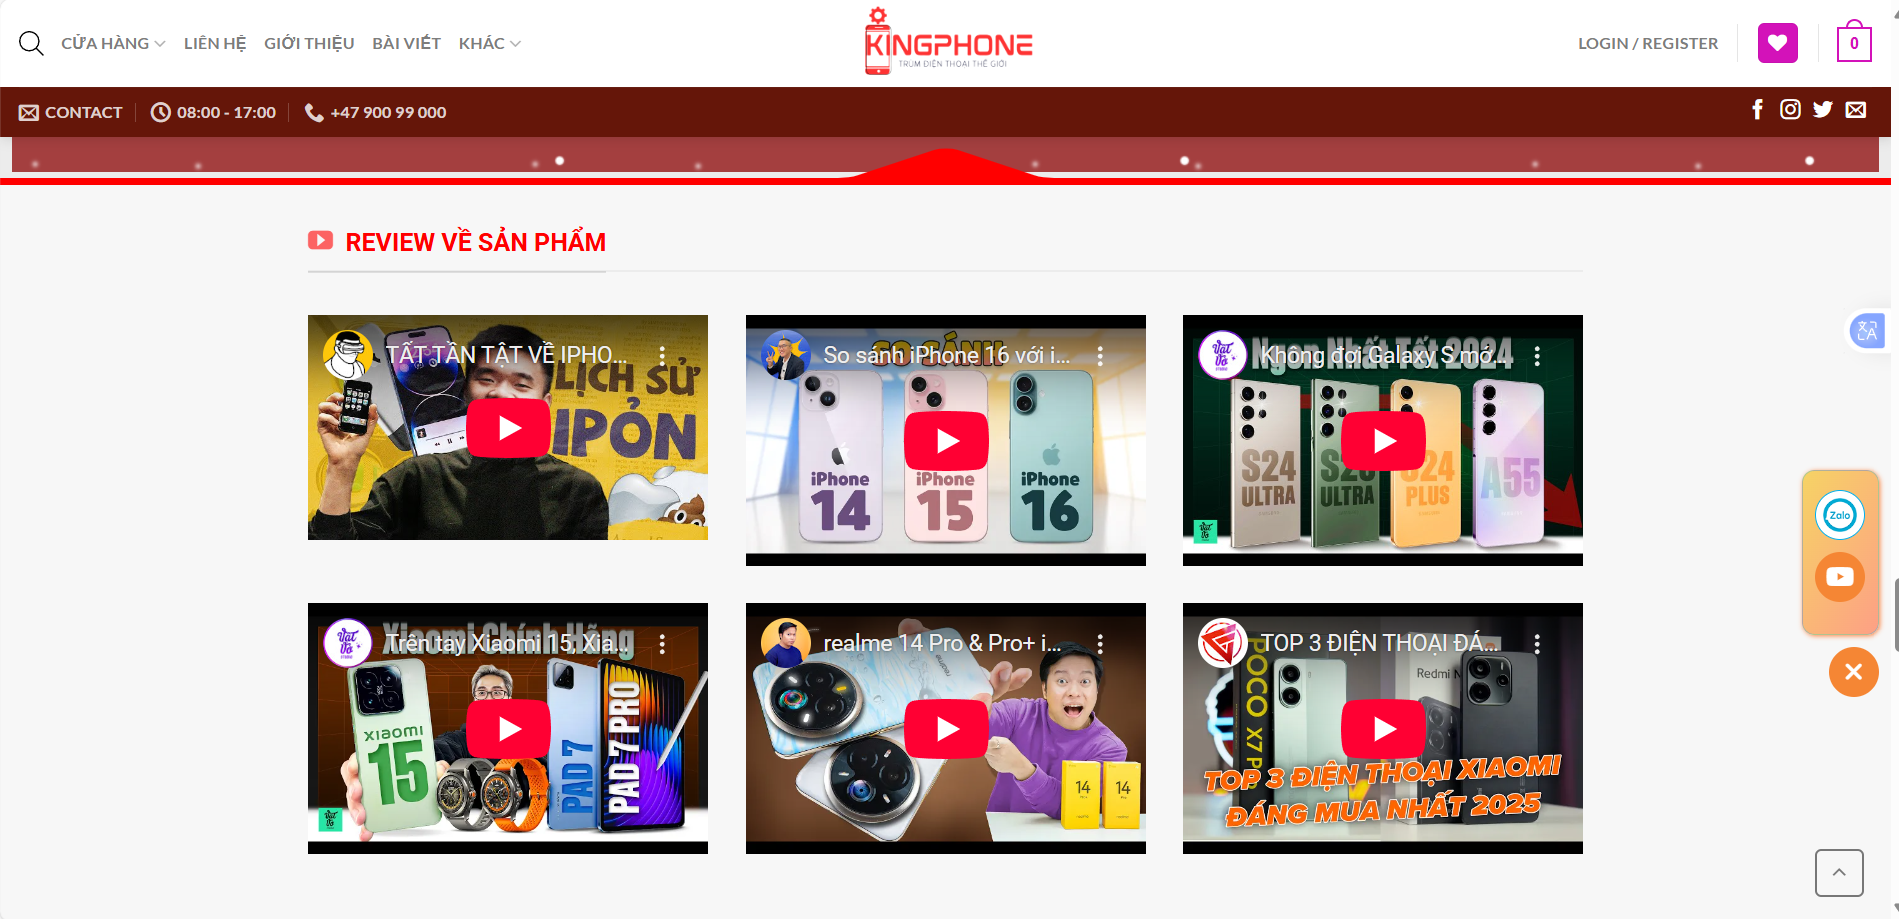
\includegraphics[width=0.6\textwidth]{img/reviewsp.png}
    \caption{Trang Reviews sản phẩm }
    \label{fig:rv}
\end{figure}

\subsubsection{Trang sản phẩm yêu thích}
\begin{figure}[H]
    \centering
    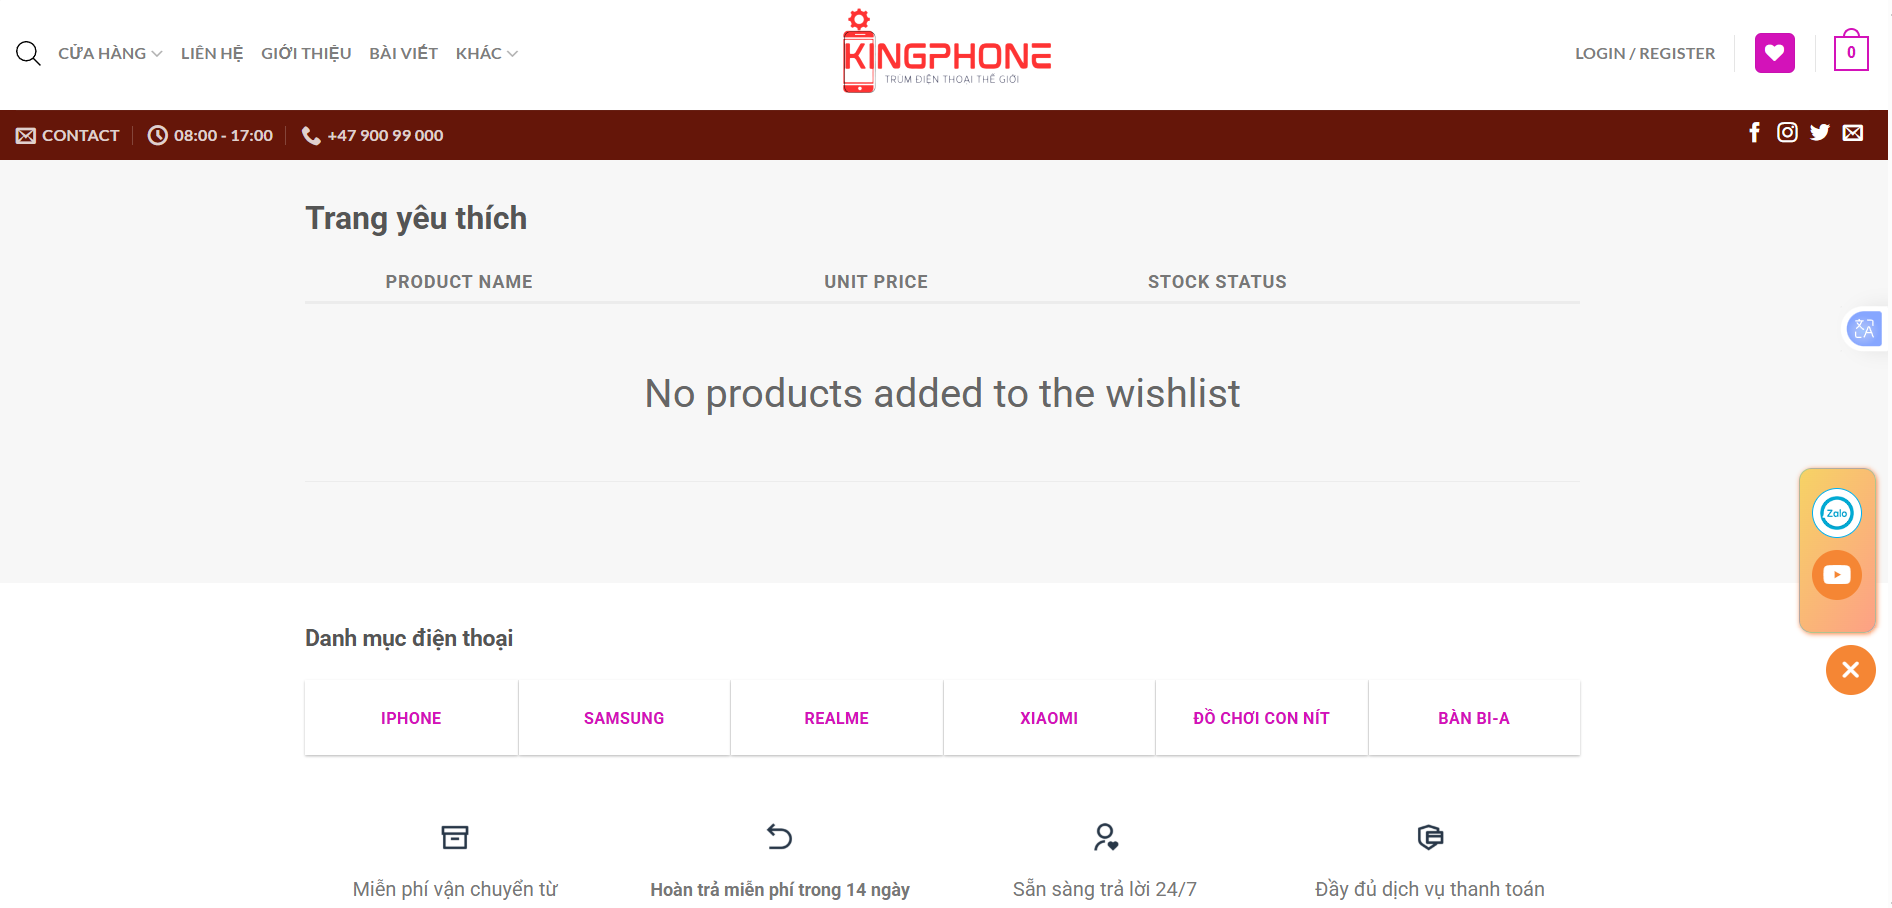
\includegraphics[width=0.6\textwidth]{img/sanphamyeuthich.png}
    \caption{Trang sản phẩm yêu thích}
    \label{fig:yeu}
\end{figure}

\subsubsection{Trang giỏ hàng}
\begin{figure}[H]
    \centering
    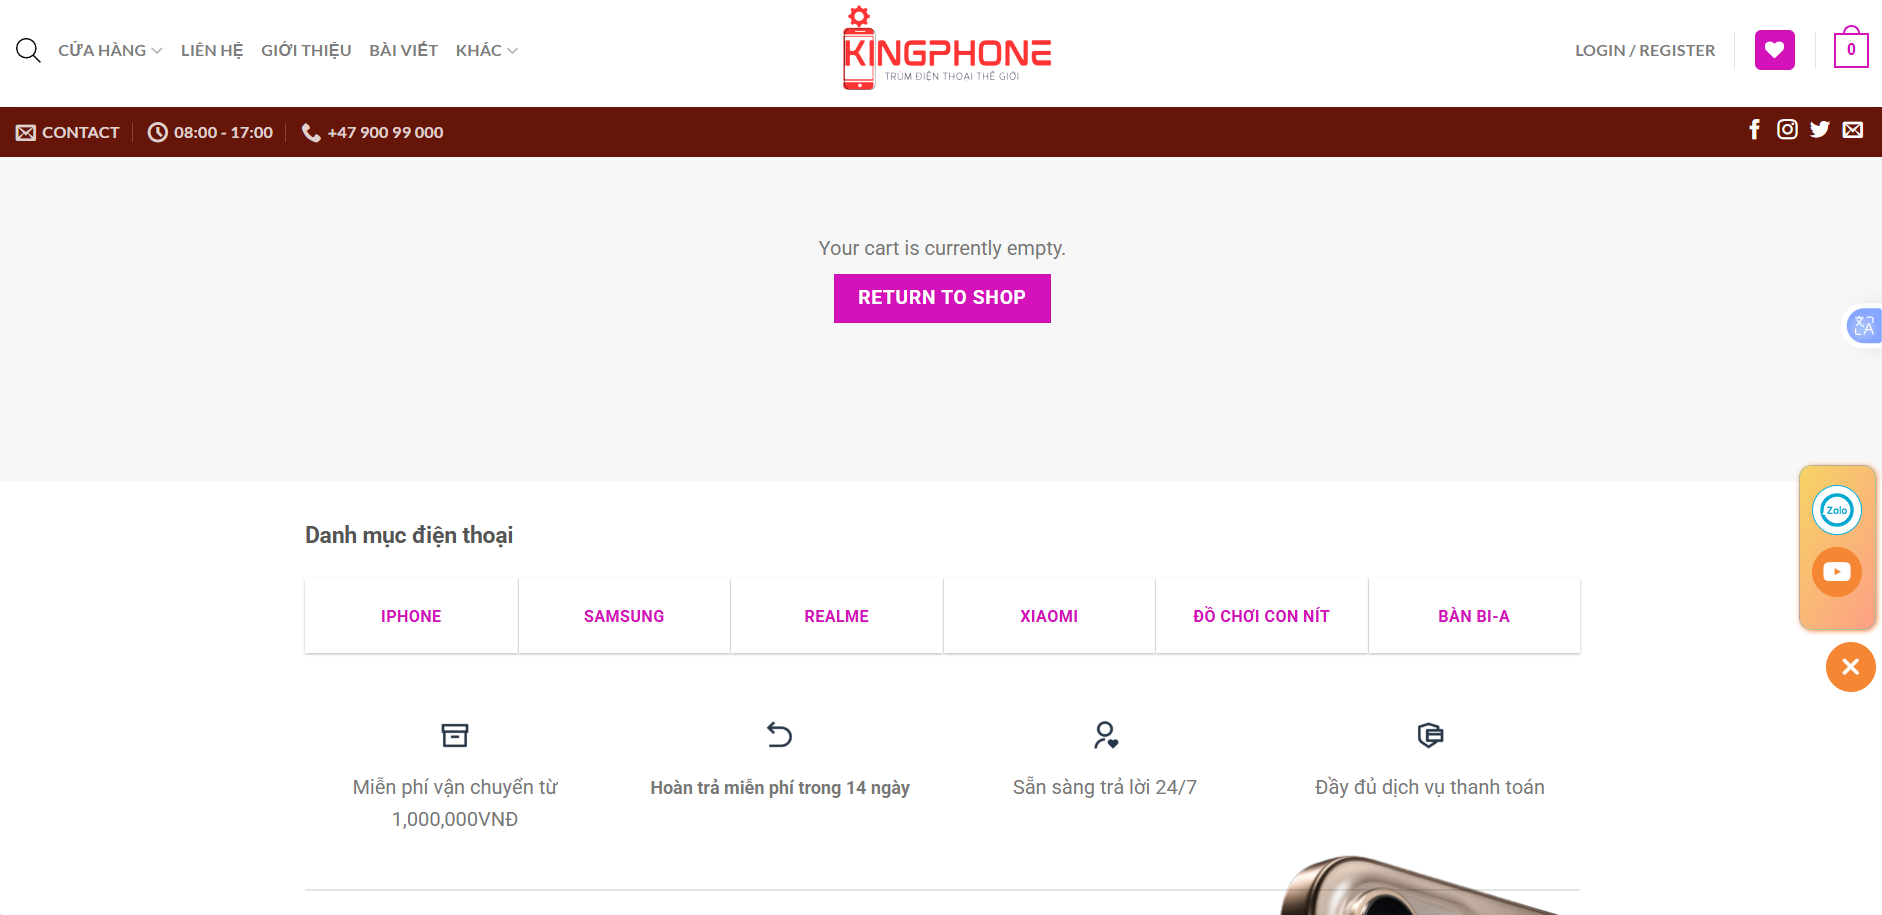
\includegraphics[width=0.6\textwidth]{img/giohang.png}
    \caption{Trang giỏ hàng}
    \label{fig:giohang}
\end{figure}

\subsubsection{Trang liên hệ}
\begin{figure}[H]
    \centering
    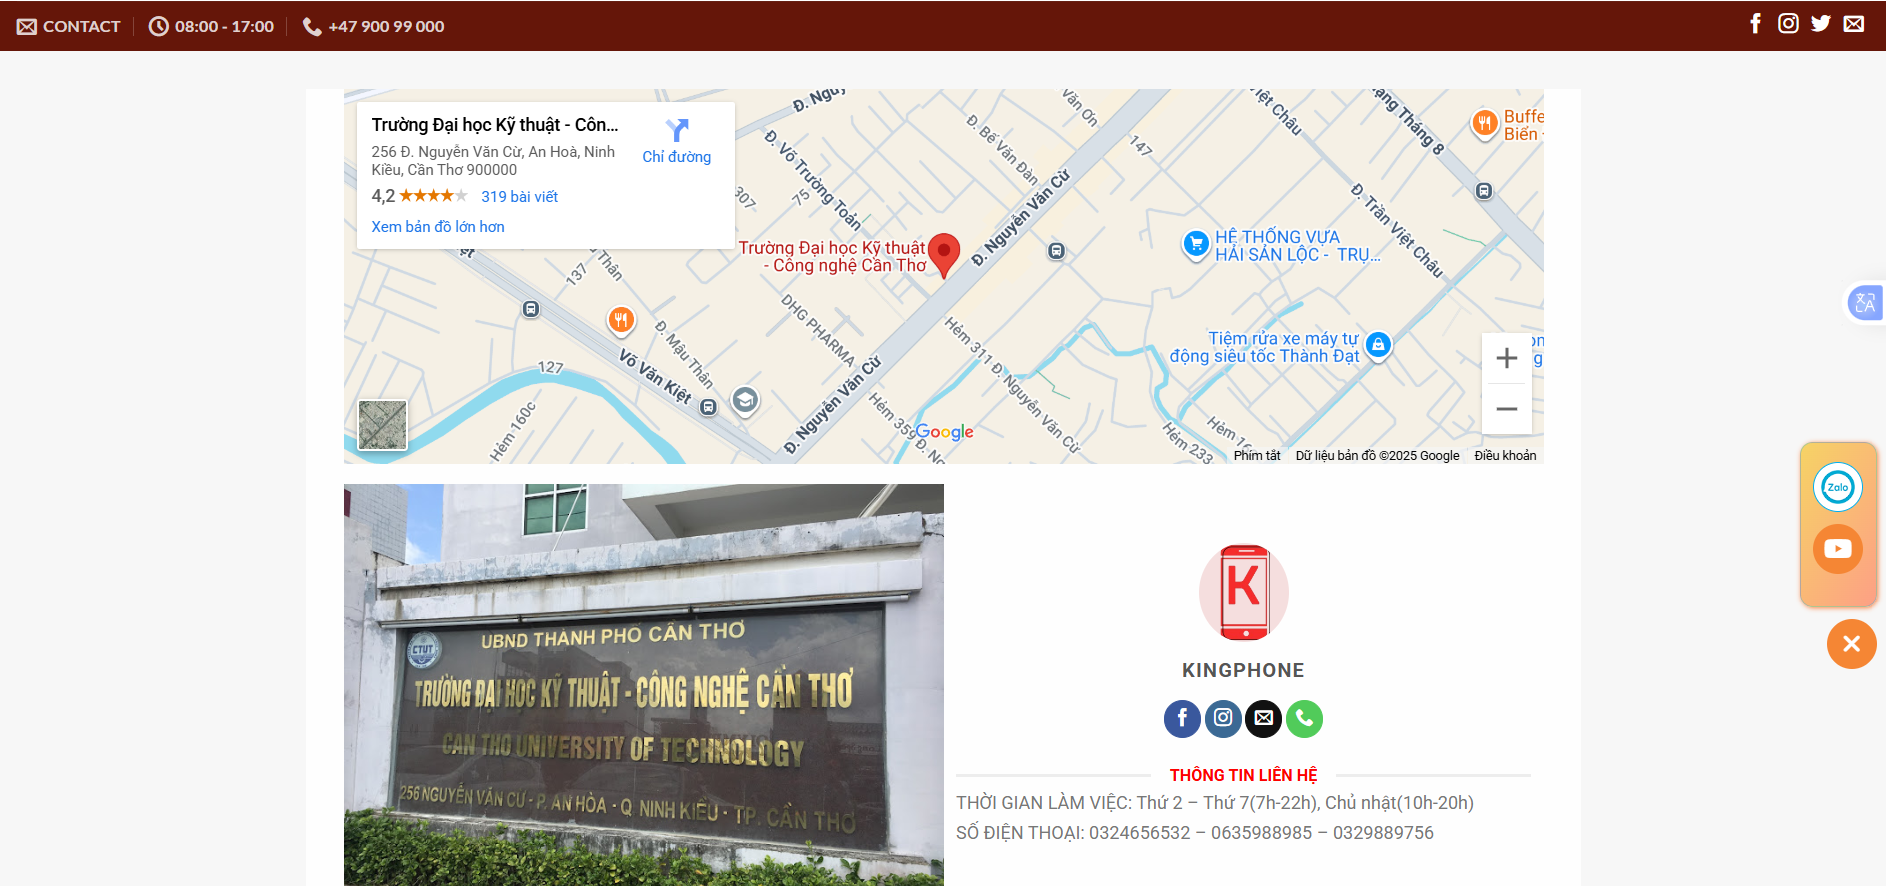
\includegraphics[width=0.6\textwidth]{img/lienhe.png}
    \caption{Trang liên hệ}
    \label{fig:lh}
\end{figure}

\subsubsection{Trang liên hệ}
\begin{figure}[H]
    \centering
    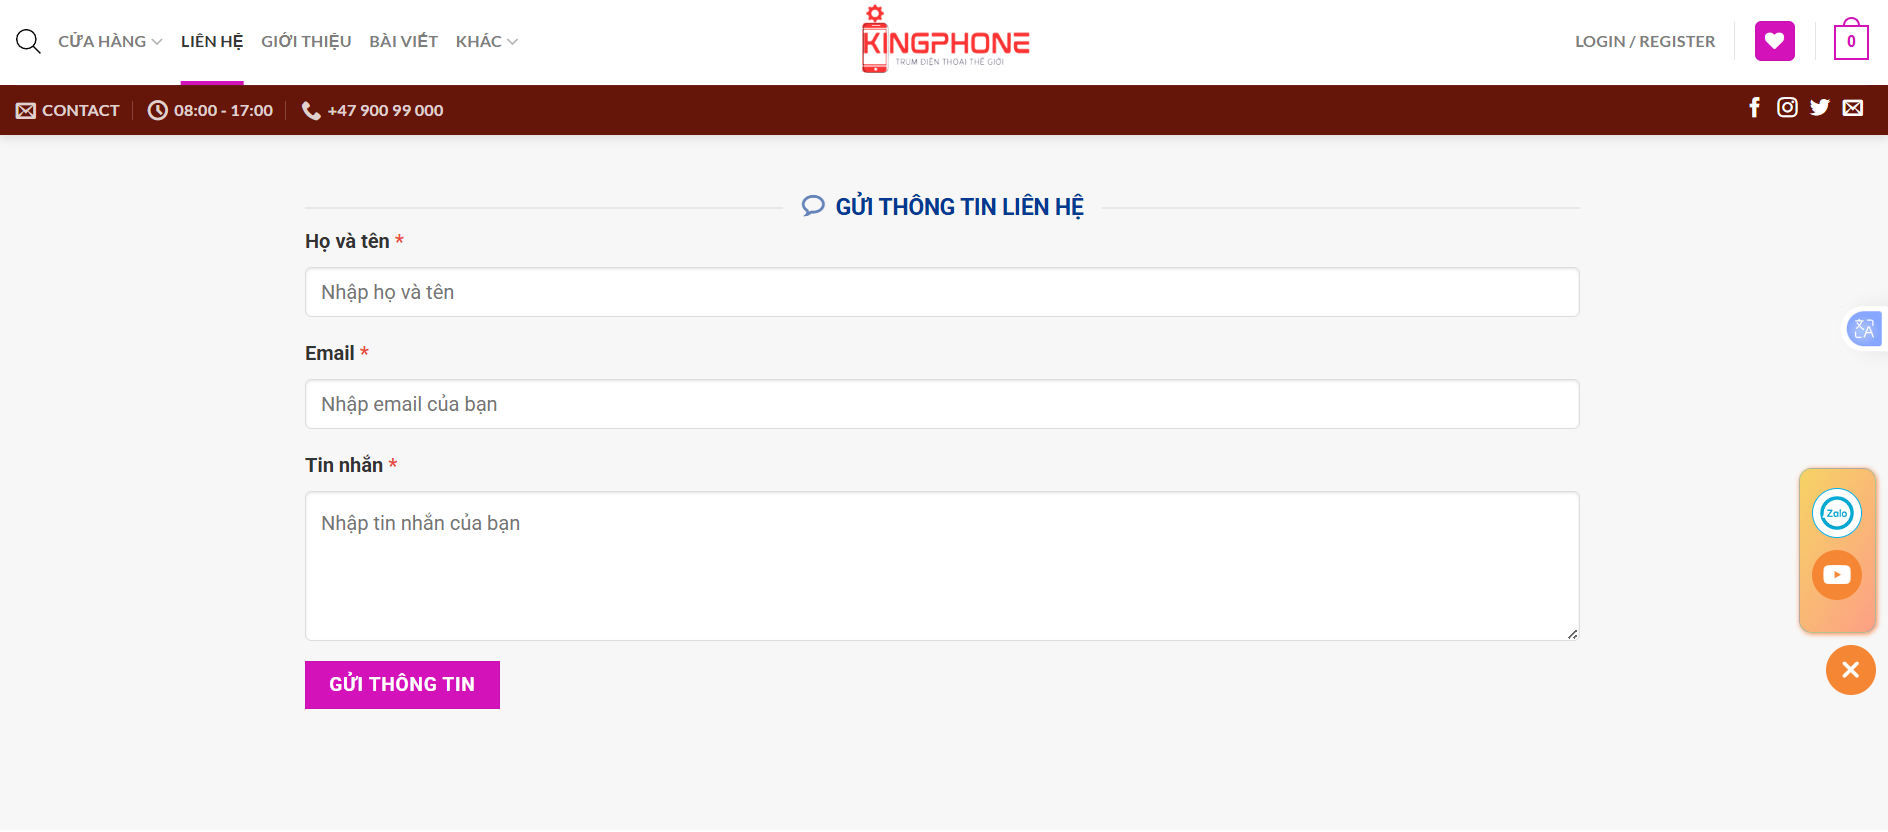
\includegraphics[width=0.6\textwidth]{img/guithongtinlienhe.png}
    \caption{Trang gửi thông tin liên hệ}
    \label{fig:noibat}
\end{figure}

\subsubsection{Trang giới thiệu}
\begin{figure}[H]
    \centering
    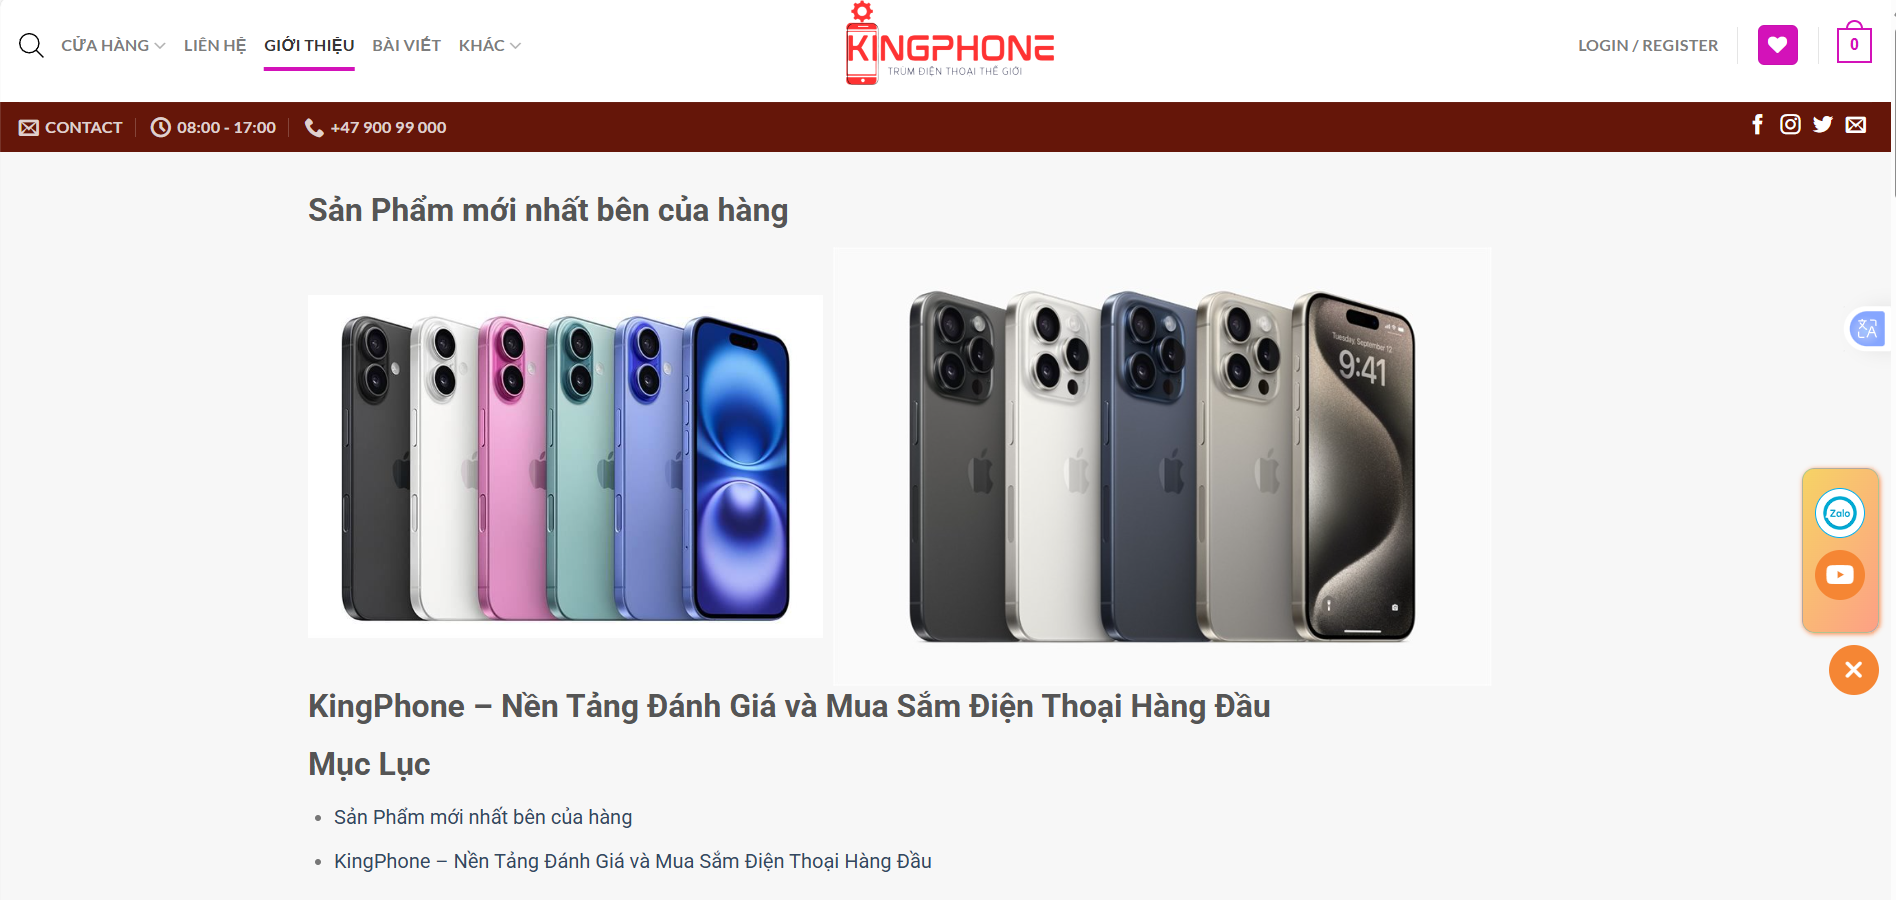
\includegraphics[width=0.6\textwidth]{img/gioithieu.png}
    \caption{Trang giới thiệu}
    \label{fig:gt}
\end{figure}

\subsubsection{Trang bài viết}
\begin{figure}[H]
    \centering
    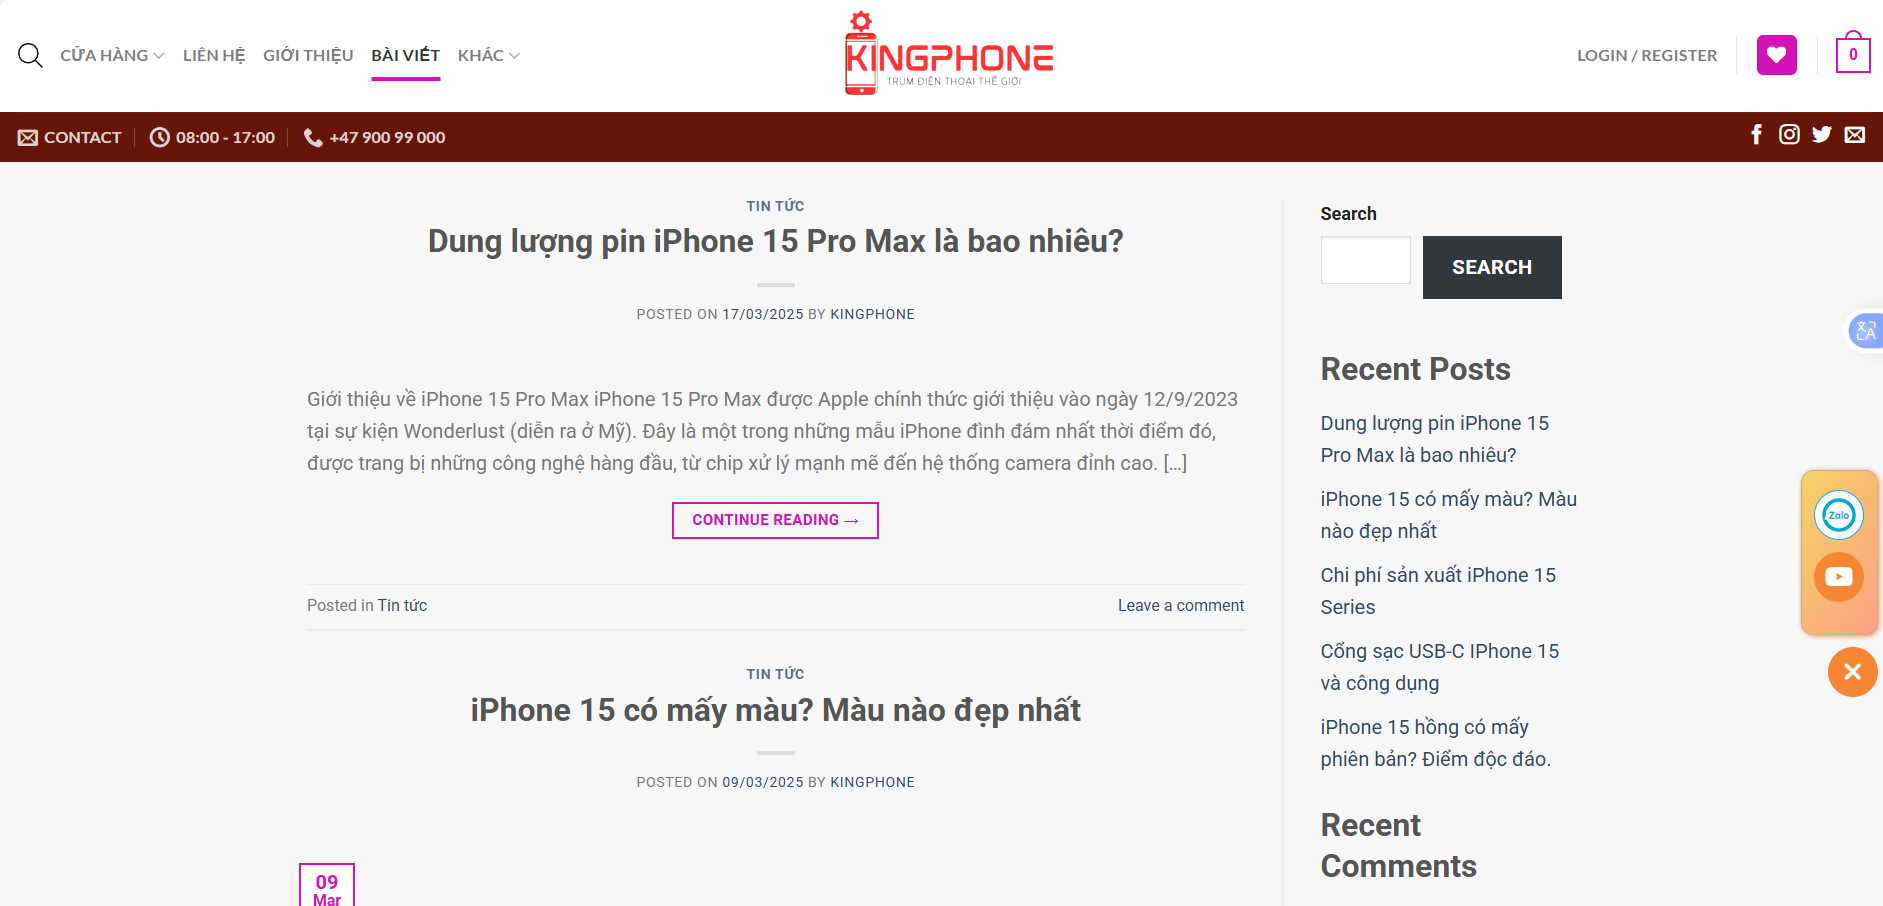
\includegraphics[width=0.6\textwidth]{img/baiviet.png}
    \caption{Trang bài viết}
    \label{fig:baiviet}
\end{figure}

\subsubsection{Trang bảo mật}
\begin{figure}[H]
    \centering
    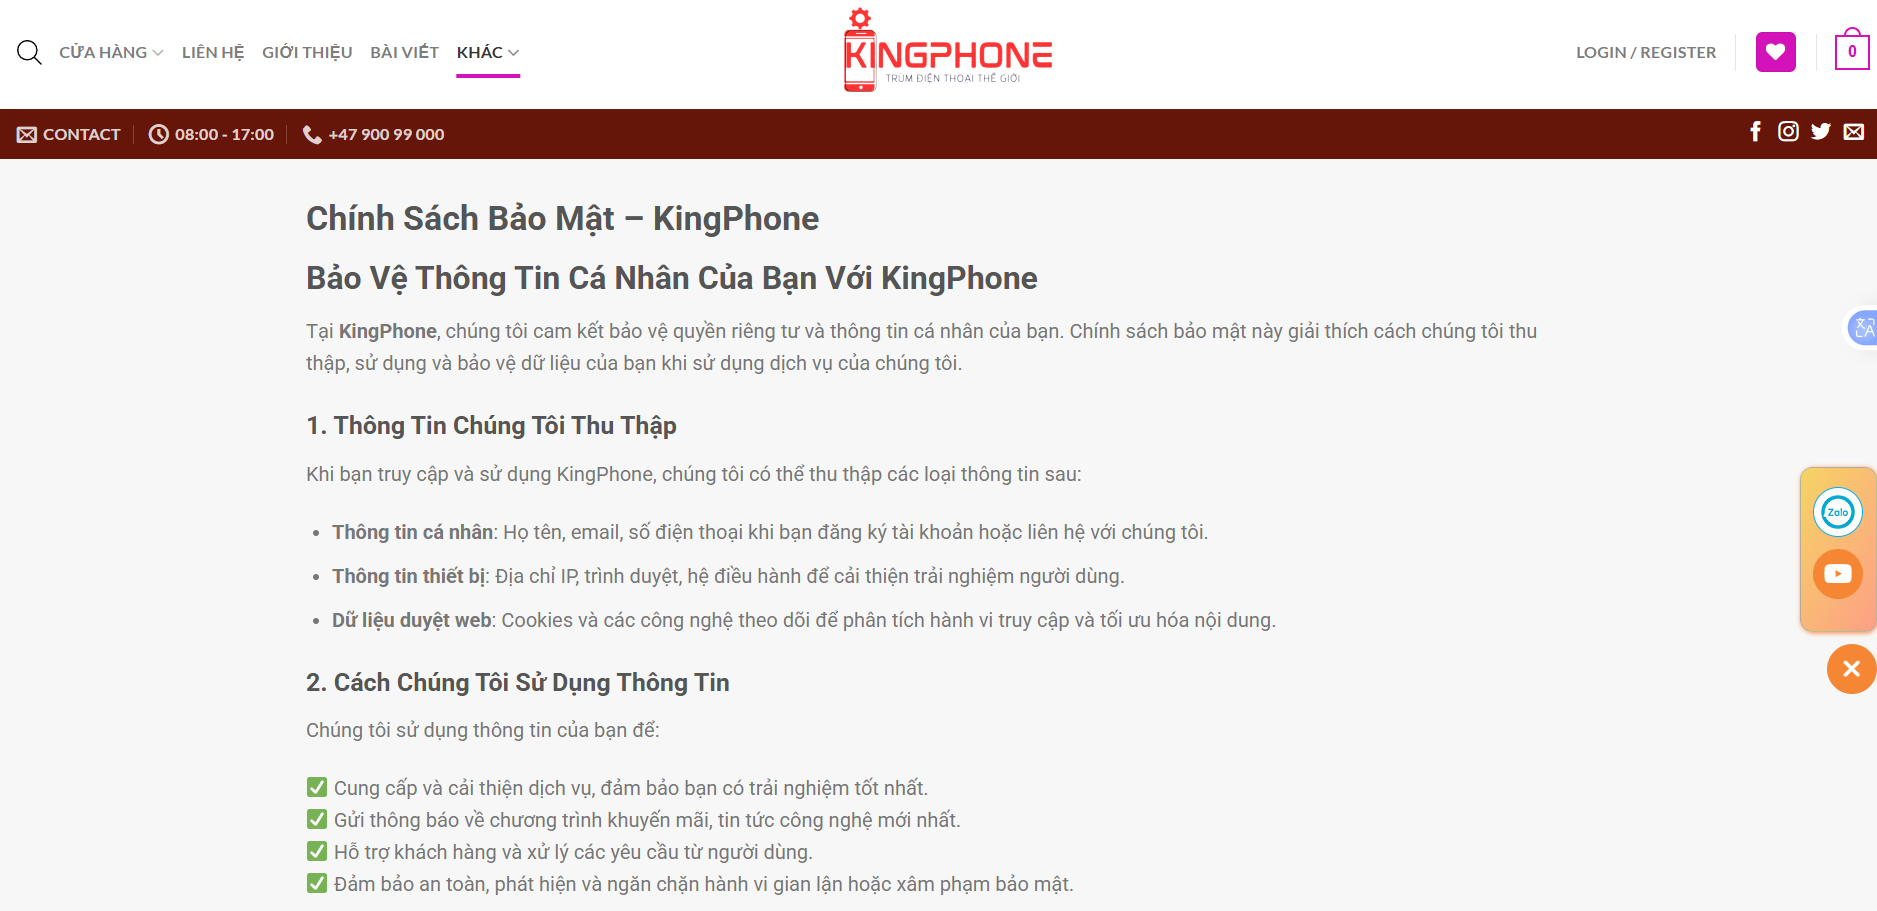
\includegraphics[width=0.6\textwidth]{img/baomat.png}
    \caption{Trang bảo mật}
    \label{fig:bmat}
\end{figure}

\subsubsection{Trang điều khoản}
\begin{figure}[H]
    \centering
    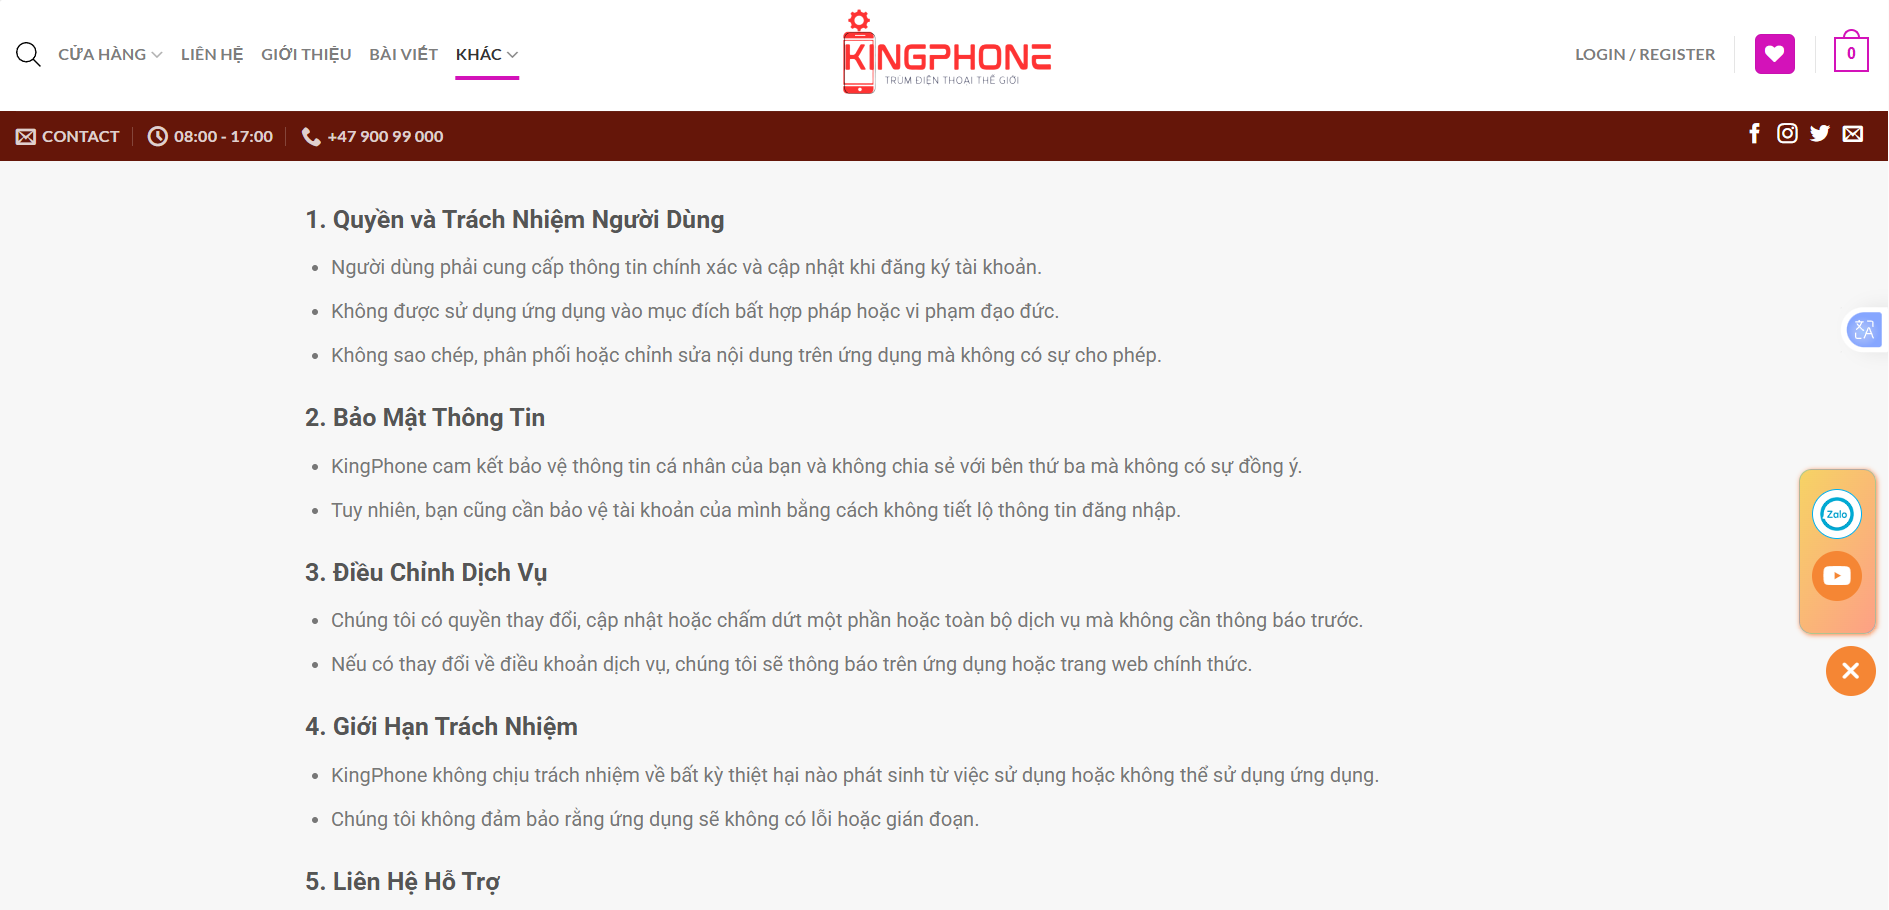
\includegraphics[width=0.6\textwidth]{img/dieukhoan.png}
    \caption{Trang điều khoản}
    \label{fig:dkhoan}
\end{figure}

\subsubsection{Trang tìm kiếm}
\begin{figure}[H]
    \centering
    
\includegraphics[width=0.6\textwidth]{img/timkiem.png}
    \caption{Trang tìm kiếm}
    \label{fig:tkiem}
\end{figure}

\section*{Kết luận chương}
Qua quá trình thực tập và triển khai đề tài, tôi đã hiểu rõ hơn về tầm quan trọng
của việc ứng dụng công nghệ tự động hóa trong hoạt động truyền thông và thương mại
điện tử. Hệ thống Chatbot Zalo đã chứng minh được khả năng hỗ trợ hiệu quả cho
doanh nghiệp, từ tiết kiệm nguồn lực, nâng cao trải nghiệm khách hàng đến hỗ trợ
marketing. Tuy nhiên, để đạt được hiệu quả toàn diện, hệ thống cần được tiếp tục cải
tiến theo các giải pháp đã đề xuất. Đây cũng chính là hướng phát triển trong tương lai,
góp phần giúp doanh nghiệp bắt kịp xu hướng chuyển đổi số.

\chapter{KẾT LUẬN VÀ ĐỀ XUẤT KIẾN NGHỊ}
\section{Kết luận}
Sau thời gian thực tập và triển khai đề tài 
\textit{``Hệ thống Tự động hóa Truyền thông và Thương mại Điện tử cho Doanh nghiệp ứng dụng Chatbot Zalo''}, 
tôi đã hoàn thành các mục tiêu đặt ra và thu được nhiều kết quả đáng khích lệ. 
Đây không chỉ là một dự án kỹ thuật mà còn là trải nghiệm thực tiễn toàn diện, 
giúp tôi rèn luyện tư duy, kỹ năng nghề nghiệp và phong cách làm việc chuyên nghiệp. 
Những kết quả đạt được có thể tóm gọn như sau:

\begin{itemize}
    \item \textbf{Kiến thức chuyên môn:} 
    Nắm vững cách thiết kế và triển khai hệ thống tự động hóa dựa trên Make.com, n8n, WordPress, 
    Zalo API, Google Sheets/Drive, Supabase và PostgreSQL. 
    Hiểu rõ tích hợp AI để sinh nội dung (text, hình ảnh, video) và xử lý dữ liệu trong các workflow, 
    từ đó hình dung rõ hơn về hệ thống truyền thông -- TMĐT khép kín.
    
    \item \textbf{Xử lý dữ liệu và tối ưu hóa quy trình:} 
    Có kinh nghiệm triển khai pipeline tự động từ Google Sheets $\rightarrow$ AI $\rightarrow$ Make.com $\rightarrow$ WordPress/Fanpage/YouTube. 
    Quản lý dữ liệu sản phẩm/khách hàng với Supabase/Postgres, tối ưu bằng phân trang, cache, batch request để tiết kiệm chi phí API.
    
    \item \textbf{Phát triển web và quản trị hệ thống:} 
    Xây dựng và quản lý website thương mại điện tử bằng WordPress với đầy đủ chức năng bán hàng, 
    đồng bộ dữ liệu sản phẩm từ Google Sheets/Drive. 
    Triển khai plugin, theme và tối ưu UI/UX cho khách hàng.
    
    \item \textbf{Kỹ năng làm việc với Chatbot và API:} 
    Trực tiếp triển khai chatbot Zalo bằng n8n + Zalo API: tiếp nhận tin nhắn, phân loại intent, 
    phản hồi AI, gửi hình ảnh sản phẩm từ Google Drive, cung cấp menu sản phẩm. 
    Nâng cao kỹ năng lập trình API, bảo mật token và mở rộng nền tảng Zalo.
    
    \item \textbf{Kỹ năng làm việc nhóm và quản lý dự án:} 
    Áp dụng Agile/Scrum mini trong triển khai: thiết kế workflow, kiểm thử, tối ưu. 
    Rèn luyện kỹ năng phân tích yêu cầu, quản lý thời gian, báo cáo tiến độ và tinh thần trách nhiệm khi làm việc nhóm.
    
    \item \textbf{Tư duy và tác phong chuyên nghiệp:} 
    Chuyển đổi tư duy từ sinh viên lý thuyết sang kỹ sư hệ thống thực tế: 
    sản phẩm phải ổn định, dễ bảo trì, bảo mật và tạo giá trị cho khách hàng. 
    Hình thành tác phong kỷ luật, chủ động học hỏi và giải quyết vấn đề.
\end{itemize}

\noindent
\textbf{Tóm lại:} Kỳ thực tập này giúp tôi trưởng thành rõ rệt về chuyên môn lẫn kỹ năng mềm, 
tự tin triển khai dự án thực tế và tích lũy nền tảng vững chắc cho sự nghiệp. 
Kết quả đạt được không chỉ đáp ứng mục tiêu học tập mà còn góp phần nhỏ vào việc xây dựng giải pháp ứng dụng thực tế 
cho doanh nghiệp vừa và nhỏ trong quá trình chuyển đổi số.

\section{Đề xuất}
Dựa trên quá trình thực hiện và kết quả đạt được, tôi đề xuất:

\begin{itemize}
    \item \textbf{Mở rộng và hoàn thiện tính năng hệ thống:}
    \begin{itemize}
        \item Tích hợp cổng thanh toán trực tuyến (Momo, VNPay, ZaloPay).
        \item Bổ sung tìm kiếm nâng cao (full-text search, Algolia/Typesense/ElasticSearch).
        \item Tăng cường chính sách khuyến mãi tự động bằng AI.
    \end{itemize}
    
    \item \textbf{Ứng dụng sâu hơn công nghệ AI/ML:}
    \begin{itemize}
        \item Phát triển hệ thống gợi ý sản phẩm thông minh (Recommendation System).
        \item Nâng cấp chatbot thành AI đa nhiệm: gợi ý sản phẩm, hỗ trợ thanh toán, xử lý khiếu nại.
        \item Ứng dụng AI để sinh báo cáo phân tích bán hàng.
    \end{itemize}
    
    \item \textbf{Tối ưu và kiểm thử diện rộng:}
    \begin{itemize}
        \item Load testing với hàng nghìn người dùng giả lập.
        \item Kiểm thử chatbot và website trên nhiều thiết bị.
        \item Tích hợp Firebase Crashlytics, Google Analytics, Supabase Monitor.
    \end{itemize}
    
    \item \textbf{Định hướng cá nhân:} 
    Sau khi tốt nghiệp, tôi mong muốn tiếp tục làm việc tại các công ty công nghệ/digital agency 
    phát triển giải pháp chuyển đổi số cho doanh nghiệp. 
    Với kinh nghiệm đã tích lũy, tôi tin rằng có thể đóng góp vào các giải pháp tự động hóa truyền thông, 
    TMĐT và ứng dụng AI/Chatbot trong kinh doanh.
\end{itemize}


\input{Chuong5}



%tài liệu tham khảo và bảng phân công nhiệm vụ

\cleardoublepage
\pagestyle{plain}
\begin{refs}
\renewcommand{\labelenumi}{[\arabic{enumi}]}
\textbf{\textit{Tiếng Anh}}
\begin{enumerate}
    \item \href{https://developers.cloudflare.com/pages/framework-guides/nextjs/deploy-a-nextjs-site/}{Cloudflare Developers. Deploy a Next.js Site. Cloudflare, 2024.}
    \item \href{https://nextjs.org/docs}{Next.js Documentation. Vercel, 2024.}
    \item \href{https://authjs.dev/getting-started/migrating-to-v5}{Auth.js Developers. Migrating to v5. Auth.js, 2024.}
    \item \href{https://developers.google.com/youtube/v3/getting-started}{Google Developers. Getting Started with YouTube Data API v3. Google, 2024.}
    \item \href{https://mui.com/material-ui/getting-started/}{MUI. Material-UI Documentation. MUI, 2024.}
    \item \href{https://blog.cloudflare.com/sending-email-from-workers-with-mailchannels}{Cloudflare Blog. Sending Email from Workers with Mailchannels. Cloudflare, 2024.}
    \item \href{https://www.cloudflare.com/learning/dns/dns-records/dns-mx-record/}{Cloudflare. DNS MX Record. Cloudflare, 2024.}
\end{enumerate}

\textbf{\textit{Tiếng Việt}}
\begin{enumerate}
    \item \href{https://thuvienphapluat.vn/}{Thư viện pháp luật.}
    \item \href{https://congtydelta.com/}{Công Ty Cổ Phần BVTV DELTA .}56
\end{enumerate}
\end{refs}


\clearpage
\phancongcongviec

\end{document}
